%*******10********20********30********40********50********60********70********80
%% ----------------------------------------------------------------
%% Thesis.tex -- MAIN FILE (the one that you compile with LaTeX)
%% ---------------------------------------------------------------- 

%% This template is based on Graduate Thesis written by Sunil Patel,
% (ho based it on the ecsthesis template) under the LaTeX Project Public License.
% which can be found here: http://latex-project.org/lppl/
% in the hope that it will be easier to use and to scale down to your needs
% by Simon Ternsjö in 2013-10



% INSTRUCTIONS:

% The meaning is not to edit this document much, but to fill in information 
% in the different files in the folders;
% Settings, Frontpages, Chapters, Appendices and possibly Files,
% as well as the file Bibliography.bib

% This template is easy to scale down to suite your need, 
% simply comment the input statements explained below


% Set up the document:
\documentclass[a4paper, 11pt, oneside]{Thesis}  % Use the "Thesis" style, based on the ECS Thesis style by Steve Gunn

% Add more package in Package.tex:
% Add your own packages here, 
% these existing packages can be removed if necessary
% not that more packages are imported in Thesis.cls, '
%  but those should not be changed if you don't know what you are doing...


\usepackage[utf8]{inputenc} % for writing other that basic characters
\usepackage{graphicx}
\usepackage{caption}
\usepackage{subcaption}
\usepackage{multicol}
\usepackage[dvipsnames*,svgnames]{xcolor}
\usepackage{listings}
\usepackage{hyperref}
\usepackage{float}
\usepackage{multirow}
\usepackage{bookmark}


% Include any extra LaTeX packages required
\usepackage[square, numbers, comma, sort&compress]{natbib}  % Use the "Natbib" style for the references in the Bibliography
\usepackage{verbatim}  % Needed for the "comment" environment to make LaTeX comments
%5%\usepackage{vector}  % Allows "\bvec{}" and "\buvec{}" for "blackboard" style bold vectors in maths

\DeclareFixedFont{\ttb}{T1}{txtt}{bx}{n}{12} % for bold
\DeclareFixedFont{\ttm}{T1}{txtt}{m}{n}{12}  % for normal
\definecolor{deepblue}{rgb}{0,0,0.5}
\definecolor{deepred}{rgb}{0.6,0,0}
\definecolor{deepgreen}{rgb}{0,0.5,0}

% Python style for highlighting
\lstset{
	backgroundcolor = \color{Ivory},
    language=Python,
    basicstyle=\footnotesize,
    otherkeywords={self},             
    keywordstyle=\footnotesize\color{deepblue},
    emph={__init__},          
    emphstyle=\footnotesize\color{deepred},    
    stringstyle=\color{deepgreen},
    frame=single,                         
    showstringspaces=false  ,
    breaklines=true,
    numbers=left,
    numberstyle=\footnotesize,
    tabsize=3,
    breakatwhitespace=false
}

% Use if you want:
%5%\graphicspath{Figures/}  % Location of the graphics files (set up for graphics to be in PDF format)
%5%\hypersetup{urlcolor=blue, colorlinks=true}  % Colours hyperlinks in blue, but this can be distracting if there are many links.

% Set your name, the title of the report and more in Administraitve.tex:
% This is where author, university, title and more is defined

% Personal information:
\newcommand{\myAuthorName}  {Andrea Spreafico}% Author Name
\newcommand{\myAuthorEmail} {asp005@post.uit.no} % Author email
\newcommand{\myTitle}       {Data Science using Python: \\ Analysis of Salmon farming in Norway} % Thesis title goes here
\newcommand{\mySubject}     {Computer Science} % Subject goes here
\newcommand{\myKeywords}    {Aquaculture, Fishery} % Keywords goes hear

% An initial approach to Data Science using Python: Analysis about Norwegian salmon farming.

% Data Science with Python for salmon farming analysis in Norway

% Data Science with Python for salmon farming prediction in Norway

% Data Science using Python: Initial analysis of salmon farming in Norway


% University information
\newcommand{\myUniversity}{University of Tromsø} %The Iniversity name goes here
\newcommand{\myUniversityWeb}{https://en.uit.no/startsida} %University Web Site URL Here (include http://
\newcommand{\myDepartment}{Department of Computer Science} % The Department goes here 
\newcommand{\myDepartmentWeb}{https://en.uit.no/om/enhet/forsiden?p_dimension_id=88138} % Department Web Site URL Here (include http://)
\newcommand{\myFaculty}{Faculty of Computer Science}
\newcommand{\myFacultyWeb}{https://uit.no/utdanning/program?p_document_id=279505}

%Degree, program or corse: ex: Master of Science, Engineering Physics
\newcommand{\myDegree}{Computer Science} % The degree, program or course-name goes here


% can be left untouched, both:
\newcommand{\myDate}{\today}
\newcommand{\myPartyalFulfillment}{A thesis submitted in partial fulfillment for the degree of Computer Science}


%% ----------------------------------------------------------------
\begin{document}

\frontmatter      % Begin Roman style (i, ii, iii, iv...) page numbering


% Here the first pages are imported, you can find them in the Frontpages folder
% Files in the subfolder Fixed does not need to be edited.
% If you don't need any of these sections, simply comment, or delete, the input-row\dfrac{•}{•}


%% All the pages before the chapters ------------------------------
% Set up the Title Page - DO NOT EDIT THIS, (if you don't want to ;)  )
% instead specify your name, title and more in "/Settings/Administrative.tex"
\title   {\myTitle}
\authors {\texorpdfstring
            {\href{\myAuthorEmail}{\myAuthorName}}
            {\myAuthorName}
         }
\addresses  {\groupname\\\deptname\\\univname}  
\date       {\myDate}
\subject    {\mySubject}
\keywords   {\myKeywords}

\maketitle
%% ----------------------------------------------------------------

\setstretch{1.3}  % It is better to have smaller font and larger line spacing than the other way round

% Define the page headers using the FancyHdr package and set up for one-sided printing
\fancyhead{}  % Clears all page headers and footers
\rhead{\thepage}  % Sets the right side header to show the page number
\lhead{}  % Clears the left side page header


%% ----------------------------------------------------------------
% Declaration Page required for the Thesis, your institution may give you a different text to place here
\pagestyle{fancy}  % Finally, implement the FancyHdr headers
\clearpage
\Declaration{

\addtocontents{toc}{\vspace{1em}}  % Add a gap in the Contents, for aesthetics

I, \myAuthorName, declare that this thesis titled, `\myTitle' and the work presented in it are my own. I confirm that:

\begin{itemize} 
\item[\tiny{$\blacksquare$}] This work was done wholly or mainly while in candidature for a research degree at this University.
 
\item[\tiny{$\blacksquare$}] Where any part of this thesis has previously been submitted for a degree or any other qualification at this University or any other institution, this has been clearly stated.
 
\item[\tiny{$\blacksquare$}] Where I have consulted the published work of others, this is always clearly attributed.
 
\item[\tiny{$\blacksquare$}] Where I have quoted from the work of others, the source is always given. With the exception of such quotations, this thesis is entirely my own work.
 
\item[\tiny{$\blacksquare$}] I have acknowledged all main sources of help.
 
\item[\tiny{$\blacksquare$}] Where the thesis is based on work done by myself jointly with others, I have made clear exactly what was done by others and what I have contributed myself.

\end{itemize}
 
\vspace{10 mm}
 
Signed:\\
\rule[1em]{25em}{0.5pt}  % This prints a line for the signature

Date:\\
\rule[1em]{25em}{0.5pt}  % This prints a line to write the date
}



% The "Funny Quote Page"
\clearpage
\pagestyle{empty}  % No headers or footers for the following pages

%use 1 or vfill to position the quote where it looks good:
\null\vfill\vfill


% Now comes the "Funny Quote", written in italics:

\textit{
    % Write a funny quote here:
    ''We did it, we bashed them, wee Potter’s the one, \\
    and Voldy’s gone moldy, so now let’s have fun!''
}
\begin{flushright}
    % If the quote is taken from someone, their name goes here:
    - Peeves
\end{flushright}


 
\vfill\vfill\vfill\vfill\vfill\null


% The Abstract Page
\clearpage 

\chapter{Abstract}

The term Data Science refers to the collection of knowledges and skills, mainly about statistics and computer science, that allow to collect, analyze and display data in order to understand actual phenomena. To extract the needed informations from the data there isn't a default technique. This study investigates about the possibility of implementing an informations extraction system using Python. This kind of systems might be used for high interest area, such as the Aquaculture industry, that is a particular relevant industry in the norwegian economy, since Norway represents the forefront of innovation and development in this area.
 





% The Acknowledgements page, for thanking everyone
\clearpage 
\chapter{Acknowledgements}

I would first like to thank my supervisor Ståle Walderhaug, for his support and for gave me the chance to write my bachelor thesis in Tromsø, which provided me extremely useful knowledge and experience.

\vspace{+0.5cm}

I would also like to express my special appreciation and thanks 

\hspace{1cm} To Bård Johan Hanssen for being always ready to help me with any kind of \hspace{1cm}problem about my thesis work.

\hspace{1cm} To Sara Björk for useful inspirations and tips. 

\hspace{1cm}  To the staff of SINTEF Nord for the given support and good times. 

\vspace{+0.5cm}
 
I take this opportunity to express gratitude to all the people that permitted me to participate at this Erasmus project in Norway, in particular:

\hspace{1cm} To my family, who always encourage and support me.

\hspace{1cm}  To the staff of my home university: Università di Milano Bicocca.

\hspace{1cm}  To the staff of my host university: UiT, Universitetet i Tromsø.

 	 
 	 
 	 




\clearpage
\setstretch{1.3} % Reset the line-spacing to 1.3 for body text (if changed)
\pagestyle{fancy} % The page style headers have been "empty" all this time, 
                  % now use the "fancy" headers as defined before
\lhead{\emph{Contents}}  % Set the left side page header to "Contents"
\tableofcontents  % Write out the Table of Contents


\setstretch{1.3} % Reset the line-spacing to 1.3 for body text (if changed)
\pagestyle{fancy} % The page style headers have been "empty" all this time, 
                  % now use the "fancy" headers as defined before
\lhead{\emph{List of Figures}}  % left side page header to "List if Figures"
\listoffigures  % Write out the List of Figures


\clearpage  % Start a new page
\setstretch{1.3} % Reset the line-spacing to 1.3 for body text (if changed)
\pagestyle{fancy} % The page style headers have been "empty" all this time, 
                  % now use the "fancy" headers as defined before
\lhead{\emph{List of Tables}}  % left side page header to "List of Tables"
\listoftables  % Write out the List of Tables


\clearpage
\pagestyle{fancy} % The page style headers have been "empty" all this time, 
                  % now use the "fancy" headers as defined before
\setstretch{1.5} % Set the line spacing to 1.5, 
                 % this makes the following tables easier to read
\lhead{\emph{Abbreviations}}  % Set the left side page header to "Abbreviations"
\listofsymbols{ll}  % Include a list of Abbreviations (a table of two columns)
{
  % \textbf{Acronym} & \textbf{W}hat (it) \textbf{S}tands \textbf{F}or \\
   \textbf{SIA} & \textbf{S}ingle \textbf{I}nput \textbf{A}nalyzer \\
   \textbf{MIA} & \textbf{M}ultiple \textbf{I}nput \textbf{A}nalyzer\\
   \textbf{ARIMA} & \textbf{A}uto\textbf{R}egressive \textbf{I}ntegrated \textbf{M}oving \textbf{A}verage\\
   \textbf{MAPE} & \textbf{M}ean \textbf{A}verage \textbf{P}ercentage \textbf{E}rror\\
   
}


% \clearpage
\pagestyle{fancy} % The page style headers have been "empty" all this time, 
                  % now use the "fancy" headers as defined before
\lhead{\emph{Physical Constants}}  %L page header to "Physical Constants"
\setstretch{1.5} % Set the line spacing to 1.5, 
                 % this makes the following tables easier to read
\listofconstants{lrcl}  % Include a list of Physical Constants 
                        % (a four column table)
{
% Constant Name & Symbol & = & Constant Value (with units) \\
Speed of Light & $c$ & $=$ & $2.997\ 924\ 58\times10^{8}\ \mbox{ms}^{-\mbox{s}}$ (exact)\\

}



% \clearpage
\pagestyle{fancy} % The page style headers have been "empty" all this time, 
                  % now use the "fancy" headers as defined before
\lhead{\emph{Symbols}}  %Left page header to "Symbols"
\setstretch{1.5} % Set the line spacing to 1.5, 
                 % this makes the following tables easier to read
\listofnomenclature{lll}  % Include a list of Symbols (a three column table)
{
% symbol & name & unit \\
$a$ & distance & m \\
$P$ & power & W (Js$^{-1}$) \\
& & \\ % Gap to separate the Roman symbols from the Greek
$\omega$ & angular frequency & rads$^{-1}$ \\
}


\clearpage
\lhead{}  % Set Left page header to nothing.
\setstretch{1.3}  % Return the line spacing back to 1.3
\pagestyle{empty}  % Page style needs to be empty for this page


\dedicatory{For/Dedicated to/To my\ldots}


\addtocontents{toc}{\vspace{2em}}  % Add a gap in the Contents, for aesthetics




%% The Body -------------------------------------------------------
\setstretch{1.3}  % Return the line spacing back to 1.3
\mainmatter	  % Begin normal, numeric (1,2,3...) page numbering
\pagestyle{fancy}  % Return the page headers back to the "fancy" style


% Include the chapters of the thesis, as separate files
% Just uncomment the lines as you write the chapters


%*******10********20********30********40********50********60********70********80

\chap{Introduction}


\section{Aim of the study}
Every single day in the world is produced a huge amount of data: some of this data, if they are analyzed and interpreted in the right way, could provide useful informations.\\
If we watch for example at the Aquaculture business in Norway is produced a big amount of data about every single locality or about national statistcs, but most of the time this data are not analyzed and difficult to understand.\\
The main purposes of this thesis are basically to test and show:
\begin{itemize} 
 \item 	Data potential in Aquaculture business in Norway through a system for analyzing and displaying data, in order to help the companies related with Aquaculture to improve their operations thanks to the analysis results.
 \item 	Python potential in data science, in order to show the people how it works and what you could do using it.
 \end{itemize}
For achieve the goals reported above, this thesis will provide:
\begin{itemize} 
 \item 	Implementation and description of a procedure that can be used for make a Python system able to do an initial analysis of  big datasets and also to display the obtained results.
 \item Implementation and description of a procedure that can be used for make a system implemented in Python able to predict future’s values using a regression model.
 
 \end{itemize}

\newpage
\section{Initial Goals}

\textbf{1) Collect as much data about aquaculture in Norway as possible.}
\vspace{-5mm}
\begin{itemize}
 \setlength{\itemsep}{-5pt}
  \item Which kind of data is possible to obtain about aquaculture general statistics in Norway? Where is possible to find it? Are that available for everyone?
  \item Which kind of data is possible to obtain about aquaculture of single locations in Norway? Where is possible to find it? Are that available for everyone?
\end{itemize}

 
\textbf{2) Increase accessibility and availability of the data.}
\vspace{-5mm}
\begin{itemize}
 \setlength{\itemsep}{-5pt}
  \item How you can create a unique dataset that contains and summarize all the data previous collected?
  \item Which kind of structure allows to the total dataset to be more accessable and readadble than the original single sources?
\end{itemize}
 
\textbf{3) Analyze and display the data.}
\vspace{-5mm}
\begin{itemize}
 \setlength{\itemsep}{-5pt}
  \item How it's possible to provide a general analysis and displaying of data about Norwegian aquaculture reported in the dataset?
  \item Which kind of Python functions is possible to use for analyze and displaying data? What is required and how is possible to implement it?
	\vspace{-3mm}
	\begin{itemize}
 	\setlength{\itemsep}{-5pt}
	\item Is Python a good programming language for data analysis and displaying?
	\item Does Python give the possibility to create analysis systems in easy way?
	 \end{itemize}
  \item Which kind of relationships and patterns about the data is possible to identify using the result graphics? How is possible to identify it?
  \item How is possible to check out the data trend line? 
  \item Which kind of informations have been reported for future reuse? How it's possible to access it? (Informations such as correlation coefficients, trend line equations,..)
 \end{itemize}


\textbf{4) Extract information from the data.}
\vspace{-5mm}
\begin{itemize}
 \setlength{\itemsep}{-5pt}
  \item Which parameters about aquaculture in Norway are increasing? How fast are they increasing/decreasing? 
  \item How you can compare different parameters trend line?
  \item Which kind of correlations is possible to find out between different parameters? How is possible to show it? What is possible to extract from that?
 \end{itemize}
 
 \newpage
 
\textbf{5) Prediction of values about the data.}
\vspace{-5mm}
\begin{itemize}
 \setlength{\itemsep}{-5pt}
  \item How is possible to predict some future values of the data that we own? 
		\vspace{-3mm}
		\begin{itemize}
 		\setlength{\itemsep}{-5pt}		
		  \item Would be useful to have the possibility of forecasting some future data?
		  \item Which kind of data might be the most useful to know for people into the Aquaculture field?
		 \end{itemize}
  \item Which Python utilities is possible to use for time series predictions?
  		\vspace{-3mm}
		\begin{itemize}
 		\setlength{\itemsep}{-5pt}	
		  \item How Python works for time series prediction systems implementation?
		  \item Which kind of accuracy it provides about the predicted values?
		  \item Would it be a good way for let the people get some experience with the machine learning field? 
		\end{itemize}
 \end{itemize}

\textbf{6) Recommendations to future work and extra ideas.}
\vspace{-5mm}
\begin{itemize}
\setlength{\itemsep}{-5pt}
	\item Which kind of services is possibl to provide using the collected informations and the implemented systems?
  		\vspace{-3mm}
		\begin{itemize}
 		\setlength{\itemsep}{-5pt}	
		  	\item How you can provide the analysis system like a service?
		  	\item How you can provide the prediction system like a service?
		\end{itemize}
 \end{itemize}




 % Introduction

%*******10********20********30********40********50********60********70********80

\chap{Background Theory} 
\section{Data science}
It's really important to have a general idea about what "Data Science" means since this thesis procedure is strongly based on the classic Data Science Process.\\
We can define Data Science like a "concept to unify statistics, data analysis and their related methods" in order to understand and analyze actual phenomena with data.\\
It includes theories drawn from many field within the broad areas of mathematics, statistics, information science and computer science.

\begin{figure}[H]
	\centering
    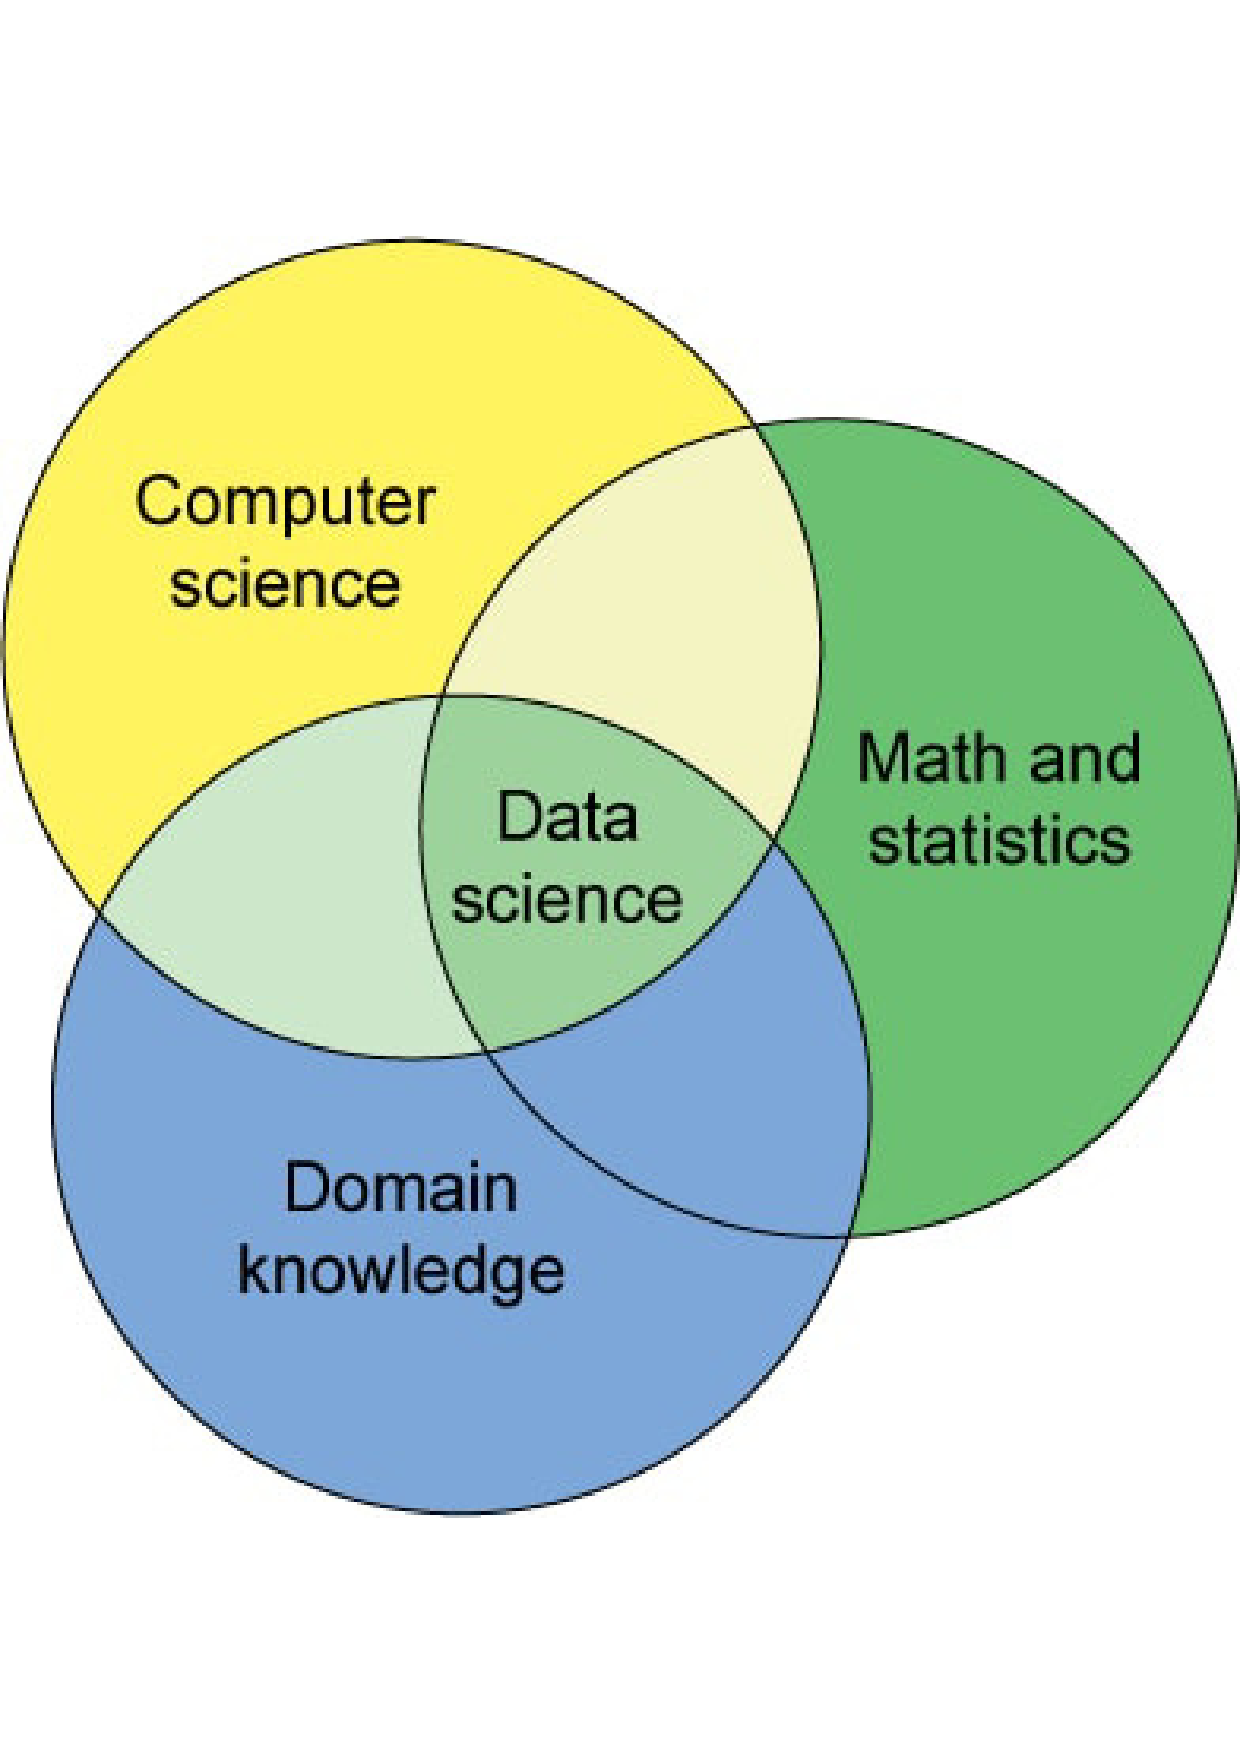
\includegraphics[trim={0 3cm 0 3cm},clip,width=0.4\textwidth]{Files/Data_Science_Concept.pdf}
    \caption{Data science concept}
    \label{fig: Data_science}
\end{figure}

\newpage

In the computer science area are particular important the subdomains of:
\begin{itemize}
\item Machine learning
\item Classification
\item Cluster Analysis
\item Data mining
\item Databases
\item Visualization
\end{itemize}

The follow image represents the "Blitzstein and Pfister's framework" and provides a clear overview of the topic.

\begin{figure}[H]
    \centering
    \makebox[\textwidth][c]{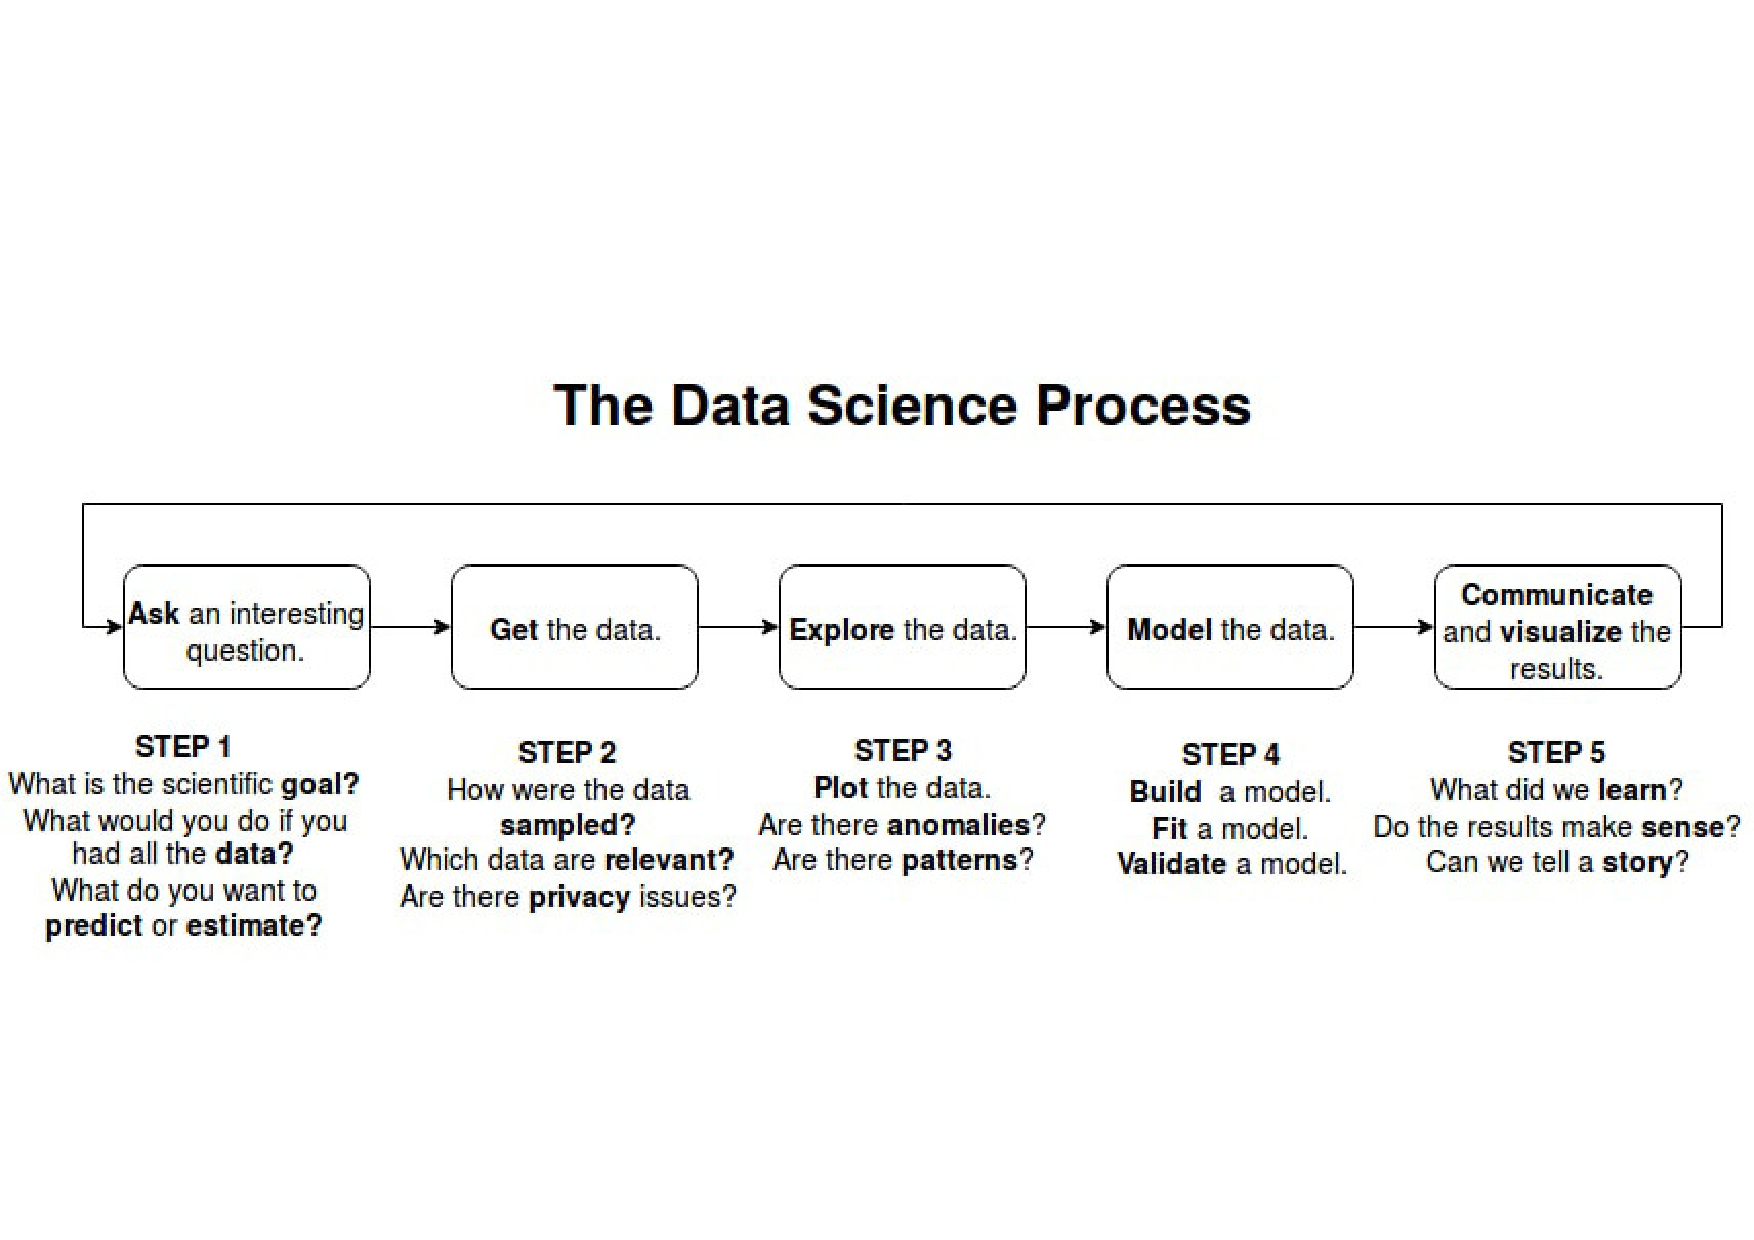
\includegraphics[trim={0 5cm 0 5cm},clip, width=1.2\textwidth]{Files/Data_Science_Process.pdf}}
    \caption[Data science process]{Data science process}
    \label{fig: Data_science}
\end{figure}



\newpage


\section{Machine learning}
This subfield of computer science gives "computers the ability to learn without being explicitly programmed". \\Evolved from the study of pattern recognition and computational learning theory in artificial intelligence, machine learning explores the study and construction of algorithms that can learn from and make predictions on data.

There are several machine learning algorithm, each one of them is used for a different purpose.The following picture gives a general idea about which categories of algorithms are used and some specific types.


\subsection{Time Series analysis and predictions}
Time Series forecasting is an important area of machine learning, but that is often neglected.

Is that important mainly beause there are so many prediction problems that involve a time component, and these problems are neglected because it is this time component that makes time series problems more difficult to handle.

" A time series is a sequence of observations taken sequentially in time. "
Quoted — Page 1, Time Series Analysis: Forecasting and Control.

Classic example of a time series dataset:\\ 		
Time \#1, observation\\
Time \#2, observation\\
Time \#3, observation

There are different goals depending on wheter we are interested in understanding a dataset or making predictions.

Understanding a dataset is called time series analysis and it can helps to make better prediction, but sometimes it's not required and can result in a large of technocal investment in time and expertise.

Making predictions could be called time series forecasting and it involves taking models fit on historical data and using them to predict future observations.

\subsection{Autoregressive integrated moving average (ARIMA)}

In statistics and econometrics, and in particular in time series analysis, an autoregressive integrated moving average (ARIMA) model is a generalization of an autoregressive moving average (ARMA) model. Both of these models are fitted to time series data either to better understand the data or to predict future points in the series (forecasting).

ARIMA(p, d, q)
\begin{itemize}
\item \textbf{p} is the number of autoregressive terms (How many preceding values are examinated for the current value’s forecast).

\item \textbf{d} is the number of nonseasonal differences needed for stationarity.

\item \textbf{q} is the number of lagged forecast errors in the prediction equation. 
\end{itemize}

\newpage

\section{Aquaculture in Norway}

Is the aquaculture business in Norway growing? 
  
Aquaculture, also known as aquafarming, is the farming of fish, crustaceans, molluscs, aquatic plants, algae, and other aquatic organisms.

Aquaculture would be the future of fish:
In 2030, according to the World Bank, aquaculture will supply:
\begin{itemize}
\item 93.6 Million tonnes of fish per year
\item 25 percent less wild fish will be available
\item 62 percent of the fish we eat will come from farms
\end{itemize}

\section{Github Usage}
GitHub is a code hosting platform for version control and collaboration. It lets you and others work together on projects from anywhere.

In this thesis it will be used like "version control" since I'm the only person working on it, and I created on myself three repositories that will be very useful for better understand the work done with this thesis.


 % Background Theory 

%*******10********20********30********40********50********60********70********80

\hypersetup{
    colorlinks=true,
    linkcolor=blue,
    filecolor=magenta,      
    urlcolor=blue,
}

% For all chapters, use the newdefined chap{} instead of chapter{}
% This will make the text at the top-left of the page be the same as the chapter

\chap{Development Method}
\section{Development Flow}

\textbf{1st Phase: Data collection and validation}\\
During this phase the most important thing is to gather as much as possible data, but they must be as much as possible reliable and useful since they are going to be indispensable for the next phases and in particular for the final results and conclusions.\\
The data’s reliability mainly depend by the kind of sources where you’re able to mine.\\
Then you should customize the unstructured data that you collected.\\
This data’s customizing has the main purposes of:
\vspace{-5mm}
\begin{itemize}
 \setlength{\itemsep}{-5pt}
 \item Let the data structure be a summarize of all the data inputs previous collected.
 \item Let the new data structure be easier to access and read.
 \item Follow some kind of setting and standard needed in the system that will be implemented.
\end{itemize}


\textbf{2nd Phase: Data Analysis and Displaying}\\
During this phase the first thing that you’re going to do is to decide some kind of analysis results that you would like to have.\\
Once you decided which kind of results you might reach, you will start with the analysis system implementation and meanwhile saving eviences of it.\\
Once the general analysis of the data is finished, and evidences have been collected, it's time to analyze it and try to extract information about it.

\newpage

\textbf{3rd Phase: Data Prediction}\\
During this phase the main purpose is to predict some kind of useful data about the current dataset. To reach this goal, is first of all indispensable to choose a prediction system to implement. \\
Once the prediction system has been implemented, it's time to apply it on the current data and try to get as much evidences as possible. \\

\textbf{4th Phase: Future Work ideas}\\
The last but not least phase is to watch at the future: try to figure out some other extra implementations about this thesis.\\


\begin{figure}[h]

    \makebox[\textwidth][c]{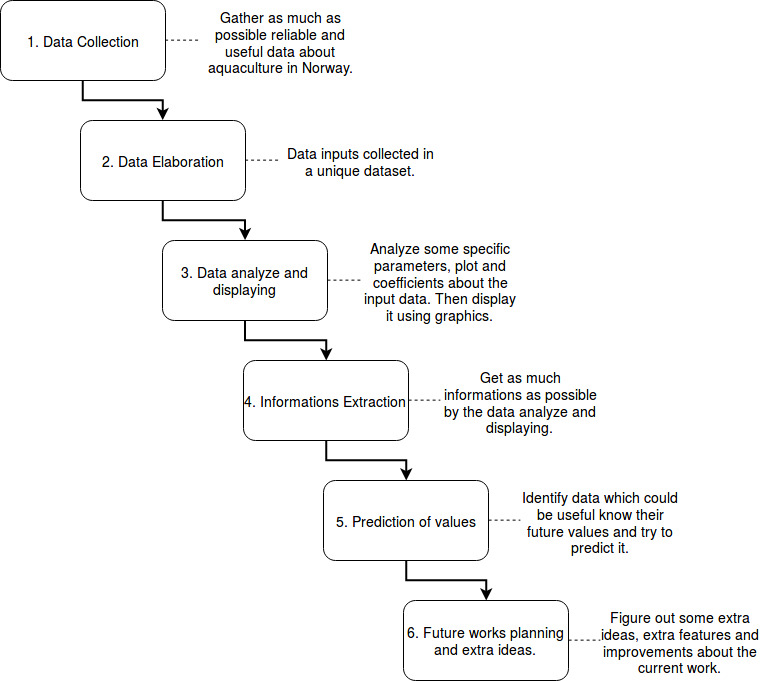
\includegraphics[width=1.2\textwidth,natwidth=761,natheight=681]{Files/DevelopmentFlow.jpg}}
    \caption[Plan flow chart]{Plan flow chart}
    \label{fig: Development_Flow}
\end{figure}

\newpage 
\section{Github Usage}
GitHub is a code hosting platform for version control and collaboration. It lets you and others work together on projects from anywhere.

In this thesis it will be used like "version control" since I'm the only person working on it, and I created on myself three repositories that will be very useful for better understand the work done with this thesis.

Repository that contains the Latex document about my thesis.\\
\url{https://github.com/Sprea22/Thesis_Latex_Doc}

Repository that contains the Data Analyzer implemented in python.\\
\url{https://github.com/Sprea22/Data_Analyzer_Python}

Repostory that contains the System for data forecasting implemented in python.\\
\url{https://github.com/Sprea22/Forecasting_System_Python}
 % Development Method


\chap{Implementation}

\hypersetup{
    colorlinks=true,
    linkcolor=blue,
    filecolor=magenta,      
    urlcolor=blue,
}

\DeclareFixedFont{\ttb}{T1}{txtt}{bx}{n}{12} % for bold
\DeclareFixedFont{\ttm}{T1}{txtt}{m}{n}{12}  % for normal
\definecolor{deepblue}{rgb}{0,0,0.5}
\definecolor{deepred}{rgb}{0.6,0,0}
\definecolor{deepgreen}{rgb}{0,0.5,0}

% Python style for highlighting
\lstset{
	backgroundcolor = \color{Ivory},
    language=Python,
    basicstyle=\footnotesize,
    otherkeywords={self},             
    keywordstyle=\footnotesize\color{deepblue},
    emph={__init__},          
    emphstyle=\footnotesize\color{deepred},    
    stringstyle=\color{deepgreen},
    frame=single,                         
    showstringspaces=false  ,
    breaklines=true,
    numbers=left,
    numberstyle=\footnotesize,
    tabsize=3,
    breakatwhitespace=false
}


\subsection{Implemented Systems repositories}
The system that is going to be implemented during this thesis can be easily downloaded in order to test it and better understandhow it works.\\
The github repository of the implementation is the following:\\
\url{https://github.com/Sprea22/Norway_County_Analyzer}\\
Direct link for the already implemented Data Analyzer in Python.\\
\url{https://codeload.github.com/Sprea22/Data_Analyzer_Python/zip/master}\\

\url{https://github.com/Sprea22/Forecasting_System_Python}\\
Direct link for the already implemented Forecasting System in Python.\\
\url{https://codeload.github.com/Sprea22/Forecasting_System_Python/zip/master}





	 % Implementation


\newpage
\chapter{Data collection}
\section{Data sources}
The collection of the data has been an important phase during this work. \\
Several sources have been checked and consulted in order to find reliable and useful data for the final purpose of this thesis.\\
In this particular case the main data collection way was internet, but some important data have been provided also from SINTEF Nord.


\subsection{Data from SINTEF Nord}
Some of the data used during this thesis were provided from the team members of the eSushi project team at SINTEF Nord. \\
The data are about each single norwegian county and with the following details:\\

\makebox[\textwidth][c]{
\resizebox{1.21\textwidth}{!}{
    \begin{tabular}{ | l | l | l | l | l |}
            \hline \textbf{Input}	&	\textbf{Content}	& \textbf{Unit}  & \textbf{Frequency}  & \textbf{Available Period} \\ \hline
\multicolumn{1}{|p{4cm}|}{\raggedright 1. Sea Average Temperature}	&	
\multicolumn{1}{p{4cm}|}{\raggedright Reported number of cages with salmon and rainbow trout.}
								& Celsius & Monthly & January 2007 - April 2014 	\\ \hline	
\end{tabular}}}




\newpage
 
\subsection{Data from Fiskeridir} 
The current website has been the main data source for this work. It provides several statistics about Aquaculture in Norway.\\
The data inputs from the current website used for this thesis are reported below, and they are available for each single county in Norway involved in Aquaculture business:

\makebox[\textwidth][c]{
\resizebox{1.2\textwidth}{!}{
    \begin{tabular}{ | l | l | l | l | l |}
            \hline
\textbf{Input}							&	\textbf{Content}	& \textbf{Unit} & \textbf{Frequency} & \textbf{Available Period} \\ \hline
1. Cages							&	\multicolumn{1}{p{4cm}|}{\raggedright Reported number of cages with salmon and rainbow trout.}
									& Number & Monthly & January 2005 - April 2017 	\\ \hline									
2. Localities						& \multicolumn{1}{p{4cm}|}{\raggedright Reported number of localities with salmon and rainbow trout.}
									& Number & Monthly & January 2007 - April 2017 \\ \hline
3. Feed consumption	&  \multicolumn{1}{p{4cm}|}{\raggedright Reported feed consumption for Salmon.}		
									& Tonnes & Monthly & January 2007 - April 2017  	\\ \hline
4. Restock			& \multicolumn{1}{p{4cm}|}{\raggedright Fish restock reported for Salmon.}	
									& 1000 pcs & Monthly & January 2007 - April 2017 	\\ \hline
5. Withdrawals 			& \multicolumn{1}{p{4cm}|}{\raggedright Withdrawals of Salmon for slaughter. } 		
									& Tonnes & Monthly & January 2007 - April 2017  	\\ \hline
6. Biomass		& \multicolumn{1}{p{4cm}|}{\raggedright Reported biomass of Salmon. }
									& Tonnes & Monthly & January 2007 - April 2017  \\ \hline
7. Salmon Number 		& \multicolumn{1}{p{4cm}|}{\raggedright Reported number of Salmon. }		
									& Number & Monthly & January 2007 - April 2017  \\ \hline
    \end{tabular}}}\\
    
    
It's also important to know that the following informations about this current data source:
\begin{itemize}
\item The data are available from 2005 to 2017.
\item The data are uploaded once per month.
\item The data are reported and available just in XLSX format.
\item The data are available just in Norwegian.
\item Is not possible to implement an automatic download script.
\end{itemize}

\newpage


\subsection{Data from Indexmundi} 
Is possible to find data about fish (salmon) monthly price, Norwegian Krone per KG.\\

\makebox[\textwidth][c]{
\resizebox{1.2\textwidth}{!}{
    \begin{tabular}{ | l | l | l | l | l |}
            \hline
\textbf{Input}	 &	\textbf{Content}	& \textbf{Unit} & \textbf{Frequency} & \textbf{Available Period} \\ \hline
\multicolumn{1}{|p{4cm}|}{\raggedright 1. Export Salmon Price}	&	
\multicolumn{1}{p{4cm}|}{\raggedright Reported farm bred Norwegian Salmon export price.}
									& NOK/KG & Monthly & January 2005 - April 2017 	\\ \hline	
\end{tabular}}}									

\section{Increase accessibility and availability of data}
In order to increase the accessibility and availability of the row data have been downloaded from the above reported sources, during this phase the main goals were:
\begin{itemize}
\item provide an accurate description (in English, since it was available just in Norwegian)
\item Report the data in a standard and reusable standard (CSV).
\item Design and build a easily readable dataset structure.
\end{itemize} 

The final decision about the datasets set up during this thesis provided the followng list of datasets, where the structure can be checked in the following two pages:
 \setlength{\itemsep}{-5pt}
\begin{itemize}
\item Overview Dataset: Norway.csv
\vspace{-2mm}
\item County 1 Dataset: Finnmark
\vspace{-2mm}
\item County 2 Dataset: Troms
\vspace{-2mm}
\item County 3 Dataset: Nordland
\vspace{-2mm}
\item County 4 Dataset: Nord Trondelag
\vspace{-2mm}
\item County 5 Dataset: Sor Trondelag
\vspace{-2mm}
\item County 6 Dataset: More og Romsdal
\vspace{-2mm}
\item County 7 Dataset: Sogn og Fjordane
\vspace{-2mm}
\item County 8 Dataset: Hordaland
\vspace{-2mm}
\item County 9 Dataset: Rogaland og Agder
\end{itemize}

\newpage

\subsubsection{Dataset about Norway}

\begin{figure}[H]
        \makebox[\textwidth][c]{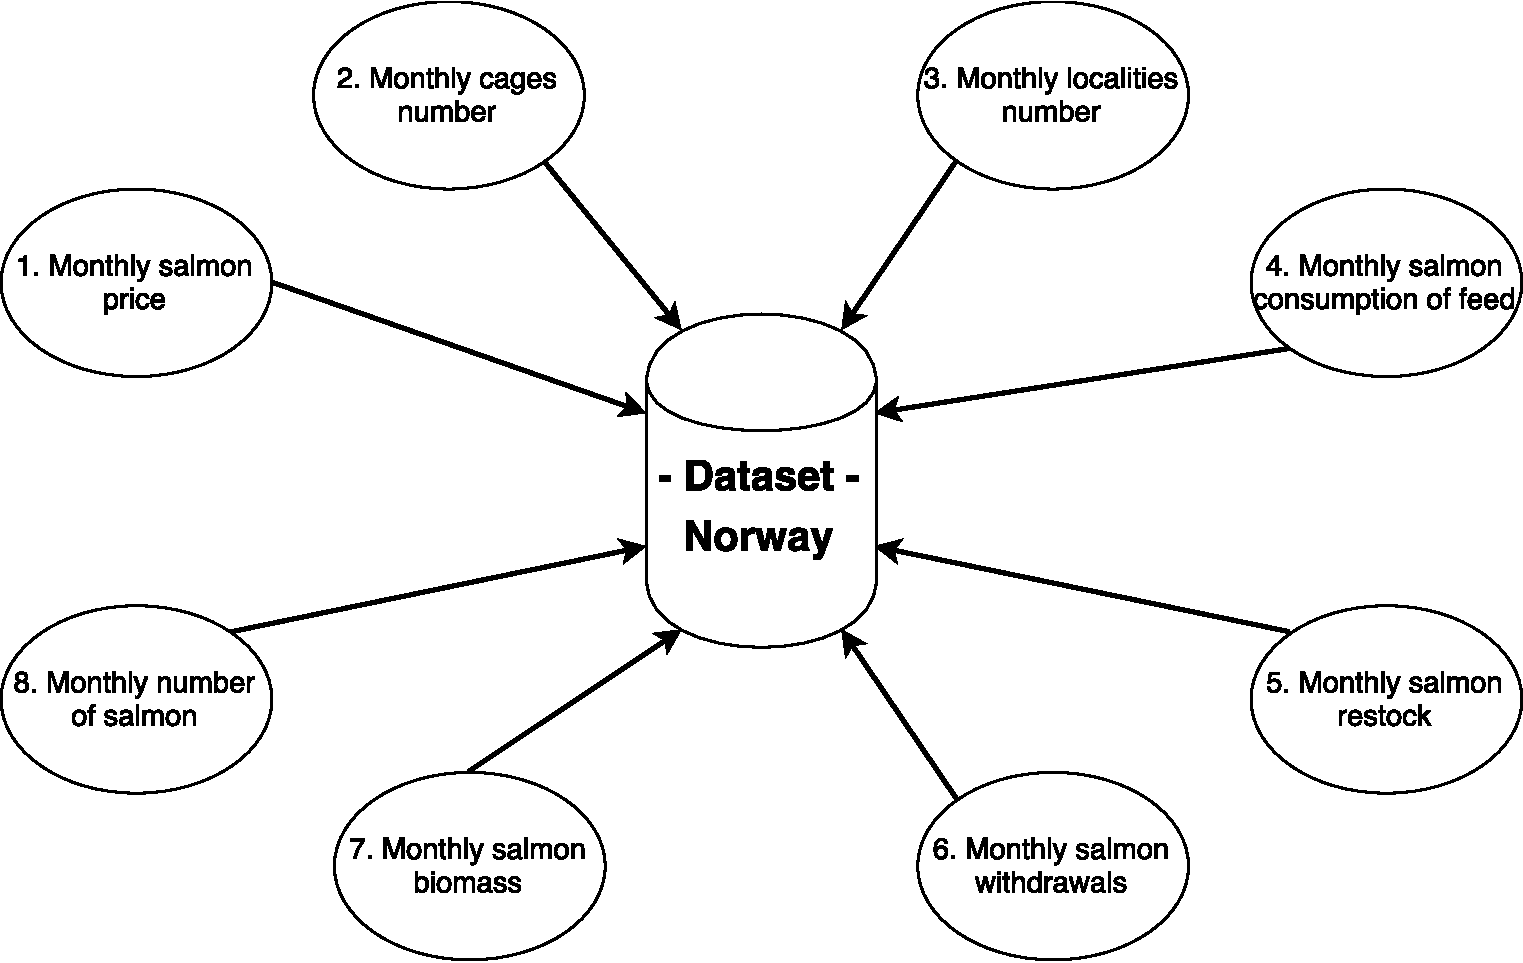
\includegraphics[width=1\textwidth]{Files/Dataset.pdf}}
    \caption{Dataset structure.}
\end{figure}

\makebox[\textwidth][c]{
\resizebox{1.2\textwidth}{!}{
    \begin{tabular}{ | l | l | l | l | }
            \hline
\textbf{Input}						& \textbf{Frequency} & \textbf{Period} & \textbf{Location}	\\ \hline
1. Export Salmon Price				& Monthly 			& January 2005 - December 2016 		& Norway 	\\ \hline	
2. Cages							& Monthly 			& January 2005 - December 2016 		& Norway 	\\ \hline									
3. Localities						& Monthly 			& January 2005 - December 2016 		& Norway	\\ \hline
4. Feed consumption					& Monthly 			& January 2005 - December 2016 		& Norway  	\\ \hline
5. Restock							& Monthly 			& January 2005 - December 2016 		& Norway	\\ \hline
6. Withdrawals 						& Monthly 			& January 2005 - December 2016 		& Norway 	\\ \hline
7. Biomass							& Monthly 			& January 2005 - December 2016 		& Norway 	\\ \hline
8. Salmon Number 					& Monthly 			& January 2005 - December 2016 		& Norway	\\ \hline
    \end{tabular}}}
    

\subsubsection{Dataset about each single county} 

\begin{figure}[H]
        \makebox[\textwidth][c]{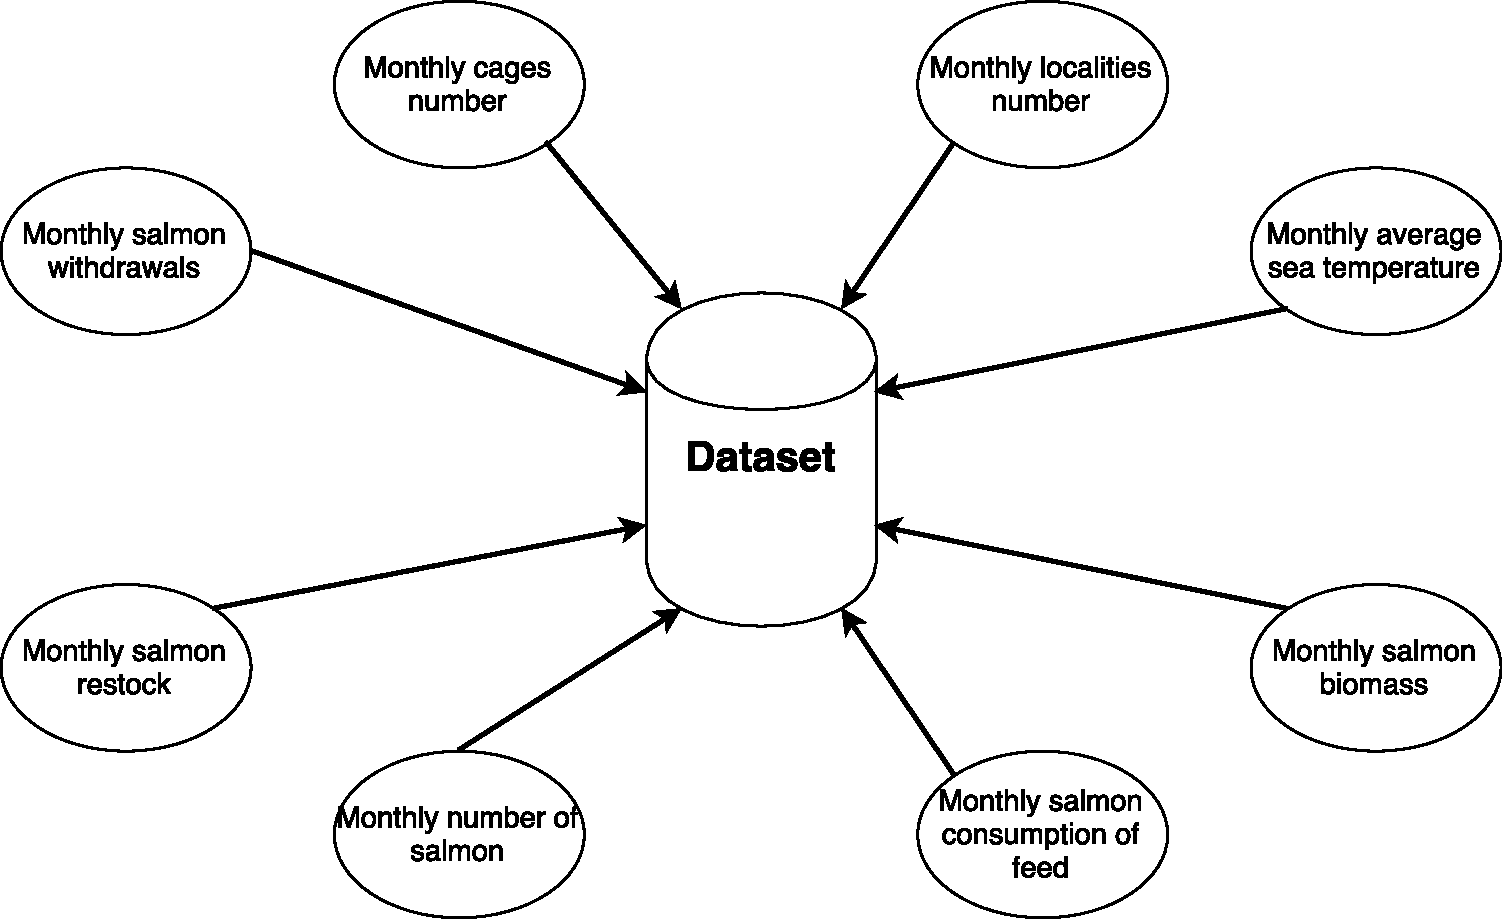
\includegraphics[width=1\textwidth]{Files/Dataset2.pdf}}
    \caption{Dataset structure.}
\end{figure}

\makebox[\textwidth][c]{
\resizebox{1.2\textwidth}{!}{
    \begin{tabular}{ | l | l | l | l | }
            \hline
\textbf{Input}						& \textbf{Frequency} & \textbf{Period} & \textbf{Location}	\\ \hline
1. Average Sea Temperature				& Monthly 			& January 2007 - December 2014 		& Single county 	\\ \hline	
2. Cages							& Monthly 			& January 2007 - December 2014 		& Single county 	\\ \hline									
3. Localities						& Monthly 			& January 2007 - December 2014 		& Single county	\\ \hline
4. Feed consumption					& Monthly 			& January 2007 - December 2014 		& Single county  	\\ \hline
5. Restock							& Monthly 			& January 2007 - December 2014 		& Single county	\\ \hline
6. Withdrawals 						& Monthly 			& January 2007 - December 2014 		& Single county 	\\ \hline
7. Biomass							& Monthly 			& January 2007 - December 2014 		& Single county 	\\ \hline
8. Salmon Number 					& Monthly 			& January 2007 - December 2014 		& Single county	\\ \hline
    \end{tabular}}}
    


\chapter{Analysis of the data}
Total implementation link for data analyzer : \\
\url{https://github.com/Sprea22/Data_Analyzer_Python}

During this part the main purpose is to analyze the whole dataset in order to find some kind of useful informations later on. 

The system that it's going to be implemented during this part of the work could be divided in two subsystems, with the relative outcomes:
\begin{itemize}
\item Single Input Analyzer (SIA): Used for analyze a single data input.
\begin{itemize}
\item Total graphic of the input data for the whole period.
\item Graphic of the input data for each single year.
\item Correlation matrix between different months of the same input.
\item Correlation matrix between different years of the same input.
\end{itemize}
\item Multiple Inputs Analyzer (MIA): Used for analyze multiple data inputs.
\begin{itemize}
\item General correlation matrix between all the different inputs.

\item Graphic of the normalized angular coefficients of all the inputs.
\end{itemize}
\end{itemize}

\newpage

\section{Requirements for reusability}
Both the analysis systems that are going to be implemented during this phase of the work will need for just one requirement about the input dataset:
\begin{itemize}
\item Monthly frequency of data values contained.
\end{itemize}

\section{System requirements}
It's important to remind that this phase can be implemented in different ways and with different programming language;\\
This proceure will describes the system implentation using Python, so be sure to have installed all the necessary for compile and execute Python code on your platform.\\
\begin{lstlisting}
Current development environment:
Python version: 2.7.12
Linux kernel version number: Linux Asus 4.4.0-71-generic SMP
\end{lstlisting}

\newpage

\section{Single Input Analyzer}
It's possible to check out the total implementation code of the SIA in the appendice  [\ref{SIA_Implementation}].
The implementation of this Analyzer can be divided in the following parts:
\begin{itemize}
\item SIA imported libraries. 
\item SIA part I: Generate and display a graphic about current input with total data.
\item SIA part II: Generate and display a graphic about current input for each year.
\item SIA part III: Generate and display a graphic that contains the correlation matrix between each single year of the current input.
\item SIA part IV: Generate and display a graphic that contains the correlation matrix between each single months of the year of the current input.
\item SIA part V: Generate and display a single overview image for the current input.
\end{itemize}

\subsection{SIA: Imported libraries}
Specific Python libraries have been imported for the implementation of this system.
It's possible to find out a list of this libraries with a specific description for each of them in the appendice [\ref{SIA_libraries}].

\newpage

\subsection{SIA section I: Total graphic for all the years}
\textbf{Goal:}\\
Generate and display the total graphic about current input, and then calculate and display the trend line as well. Trend line angular coefficient has to be save in a document.

\textbf{Requirements:}\\
The current data input has to be with a monthly frequency. 

\textbf{Implementation:}\\
To reach the current goal have been used two main functions of the "pandas" library. They allow to read the data values from the dataset and display it on a graphic.
\begin{lstlisting}
series = pandas.read_csv()
seris.plot()
\end{lstlisting}

It's possible to check out the full commented implementation in the appendice: [\ref{SIA_section_I}]

\textbf{Results:} \\
With this first part of the code has been reached the first goal of displaying and saving the basic graphic about the current input, with also the relative trend line and saving it angular coefficient in a document, that looks like:

\begin{figure}[H]
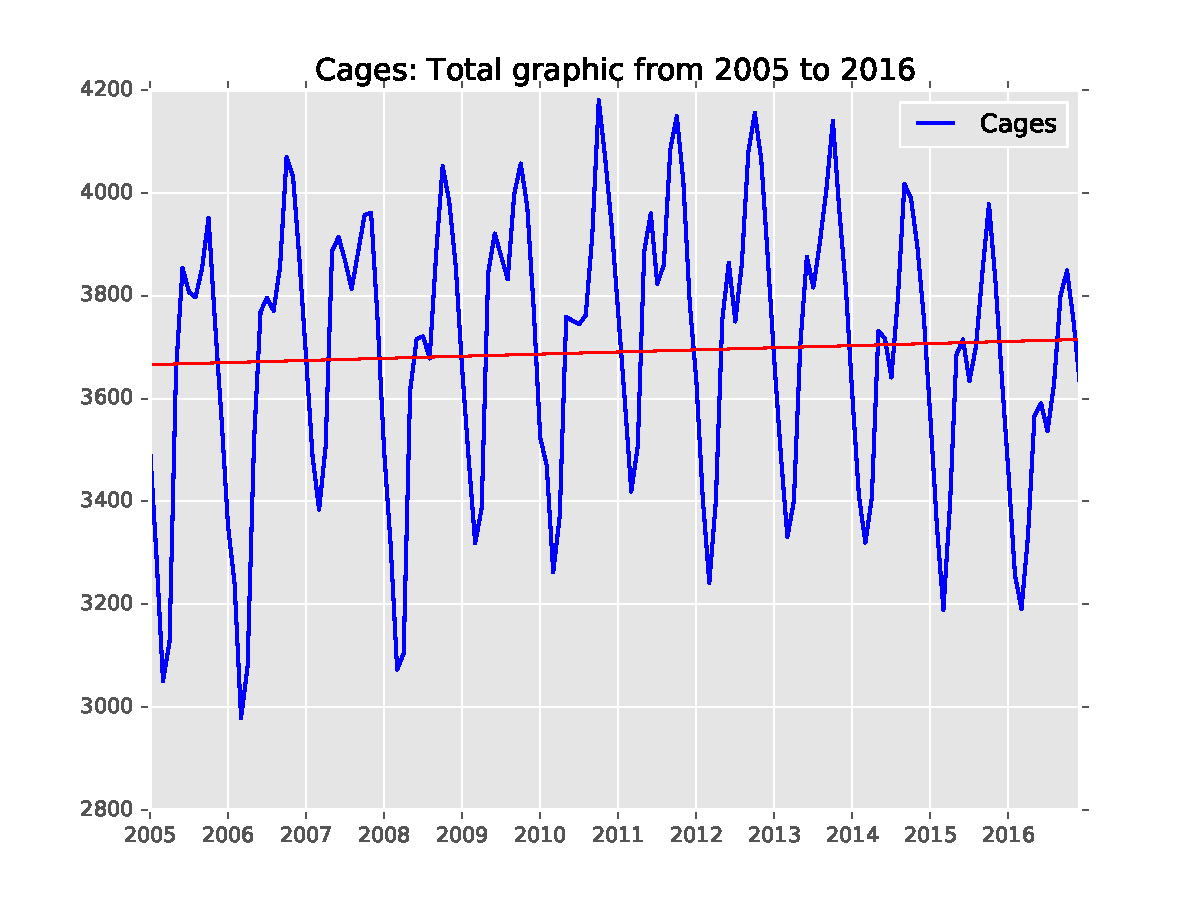
\includegraphics[width=0.9\textwidth]{Files/Cages_Total.pdf}
\caption{Total graphic about current input over the whole period.}
\end{figure}



\newpage
\subsection{SIA section II: Single graphics for each year}

\textbf{Goal:}\\
Generate and display a graphic that contains the plots of each single year over the whole period of the current input. 

\textbf{Requirements:}\\
The current data input has to be with a monthly frequency. 

\textbf{Implementation:}\\
To reach the current goal have been used two main libraries.\\
The "pandas" library allows to read the data values from the dataset and return it like "ndarray" type, then the library "pyplot" allows to display it on a graphic.
\begin{lstlisting}
series = pandas.read_csv()
series.values()
pyplot.plot()
\end{lstlisting}

It's possible to check out the full ccommented code in the appendice: [\ref{SIA_section_II}]

\textbf{Results:} \\
With this second part of the code has been reached the goal of displaying and saving the graphic of the plots for each single year of the current input, that looks like:
\begin{figure}[H]
	\centering
    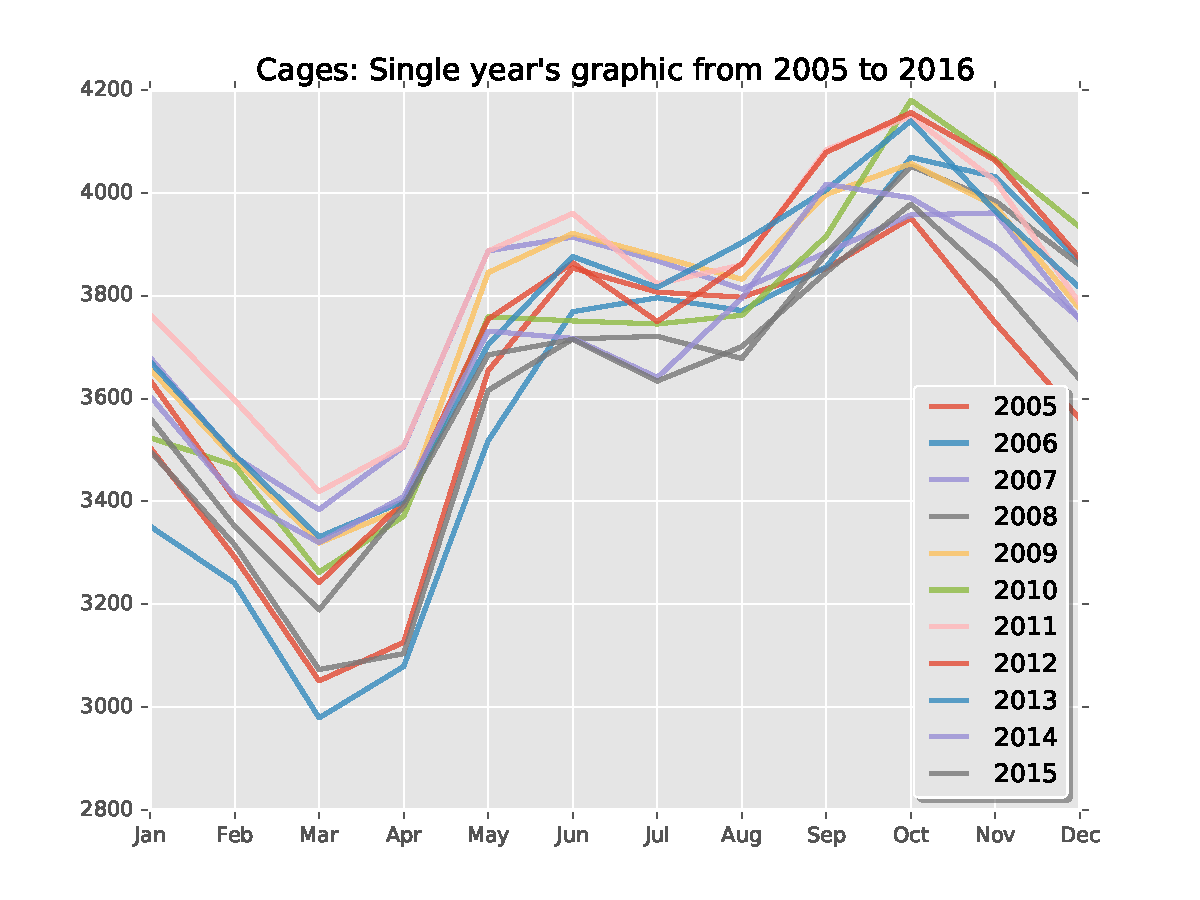
\includegraphics[width=0.9\textwidth]{Files/Cages_Years.pdf}
    \caption{Graphics for each single year of the current input data.}
\end{figure}




\newpage
\subsection{SIA section III: Correlation matrix between years}

\textbf{Goal:}\\
Calculate and save the correlation coefficients between each single year over the whole period of the current input and then display it with a correlation matrix.

\textbf{Requirements:}\\
The current data input has to be with a monthly frequency. 

\textbf{Implementation:}\\
To reach the current goal have been used the scientific computing library "numpy", that allows to calculate the correlation coefficients between data. Then the library "pyplot" has been used to display the results on a matrix.
\begin{lstlisting}
numpy.corrcoef()
figure = pyplot.figure()
ax = figure.add_subplot()
ax.matshow()
\end{lstlisting}

It's possible to check out the full ccommented code in the appendice: [\ref{SIA_section_III}]

\textbf{Results:} \\
With this part of the code have been calculated and displayed the correlation coefficients between each single year of the current input, that looks like:

\begin{figure}[H]
	\centering
    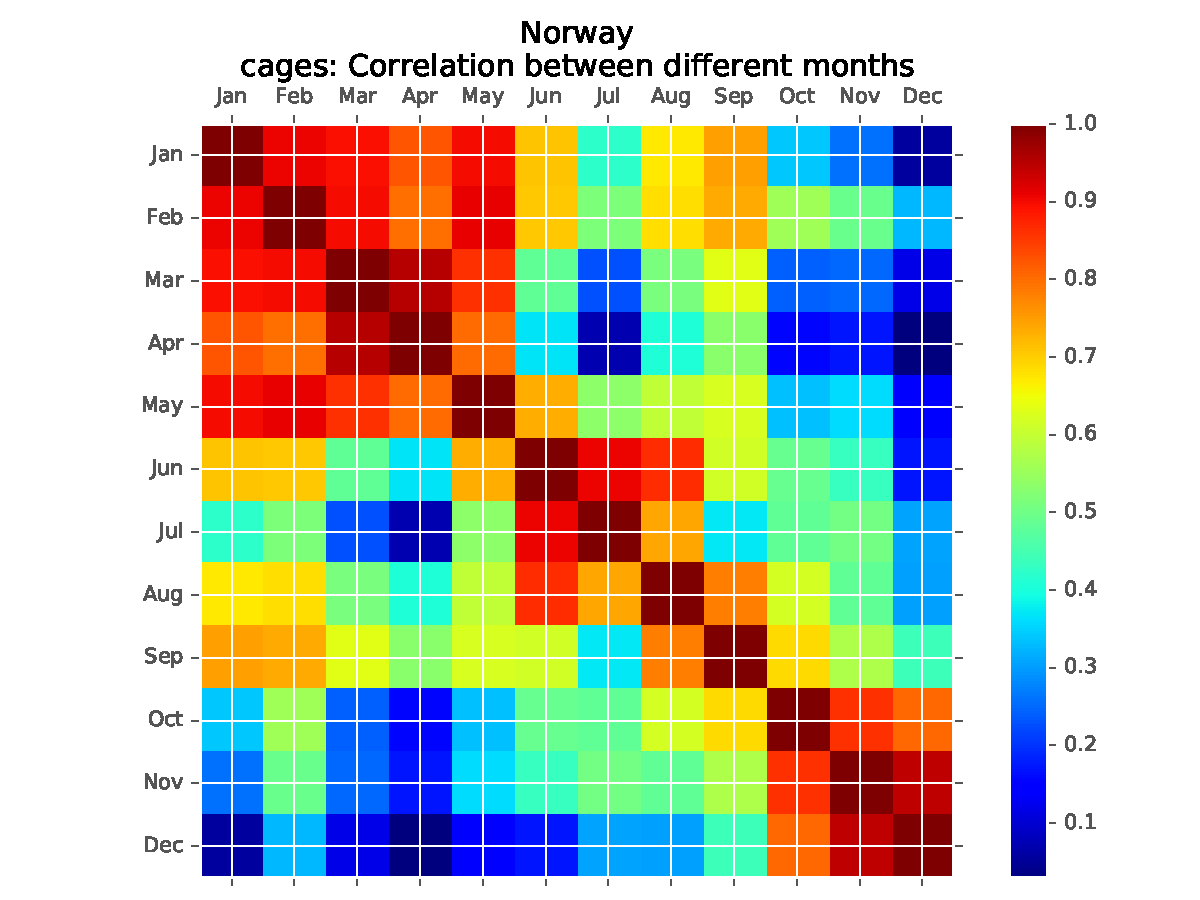
\includegraphics[width=0.9\textwidth]{Files/Cages_Months_Matrix.pdf}
    \caption{Correlation matrix between different months of the same input}
\end{figure}




\newpage
\subsection{SIA section IV: Correlation matrix between months}

\textbf{Goal:}\\
Calculate and save the correlation coefficients between each single month of the current input and then display it with a correlation matrix.

\textbf{Requirements:}\\
The current data input has to be with a monthly frequency. 

\textbf{Implementation:}\\
To reach the current goal have been used the scientific computing library "numpy", that allows to calculate the correlation coefficients between data. Then the library "pyplot" has been used to display the results on a matrix.
\begin{lstlisting}
numpy.corrcoef()
figure = pyplot.figure()
ax = figure.add_subplot()
ax.matshow()
\end{lstlisting}

It's possible to check out the full ccommented code in the appendice: [\ref{SIA_section_IV}]


\textbf{Results:} \\
With this part of the code have been calculated and displayed the correlation coefficients between each single month of the current input, that looks like: 

\begin{figure}[H]
	\centering
    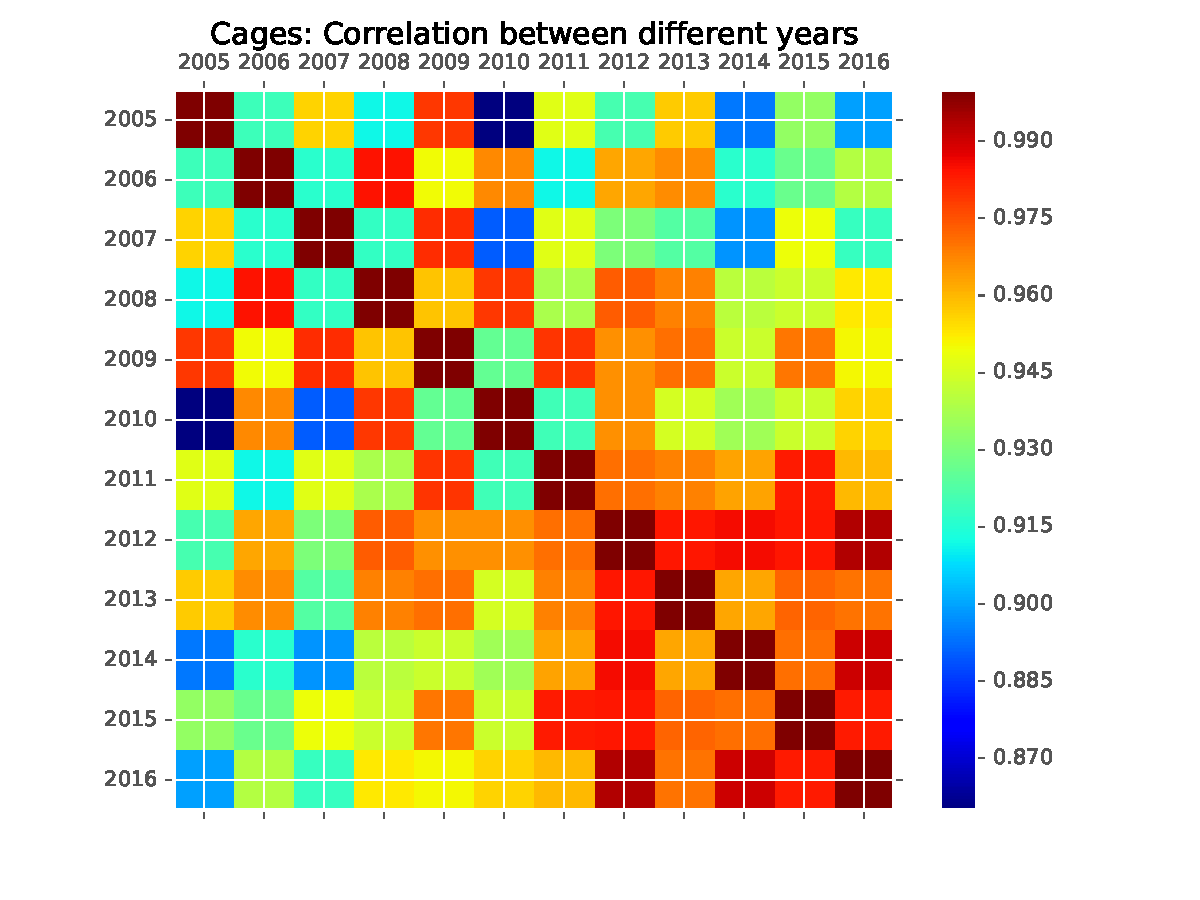
\includegraphics[width=0.9\textwidth]{Files/Cages_Years_Matrix.pdf}
    \caption{Correlation matrix between different years of the same input}
\end{figure}


\newpage
\subsection{SIA section V: Single overview}

\textbf{Goal:}\\
Generate and display a single overview image that contains all the graphics previous calculated for the current input.

\textbf{Implementation:}\\
It's possible to check out the full ccommented code in the appendice: [\ref{SIA_section_V}]

\textbf{Requirements:}\\
- All the graphics about the current input have to be already calculated and saved.

\textbf{Results:}
With this part of the code it's possible to have a single overview image for the current input, that is basically showing and comparing all the graphics that have already been calculated about this input. It looks like this example:



\begin{figure}[H]
\begin{subfigure}{.5\textwidth}
	\centering
    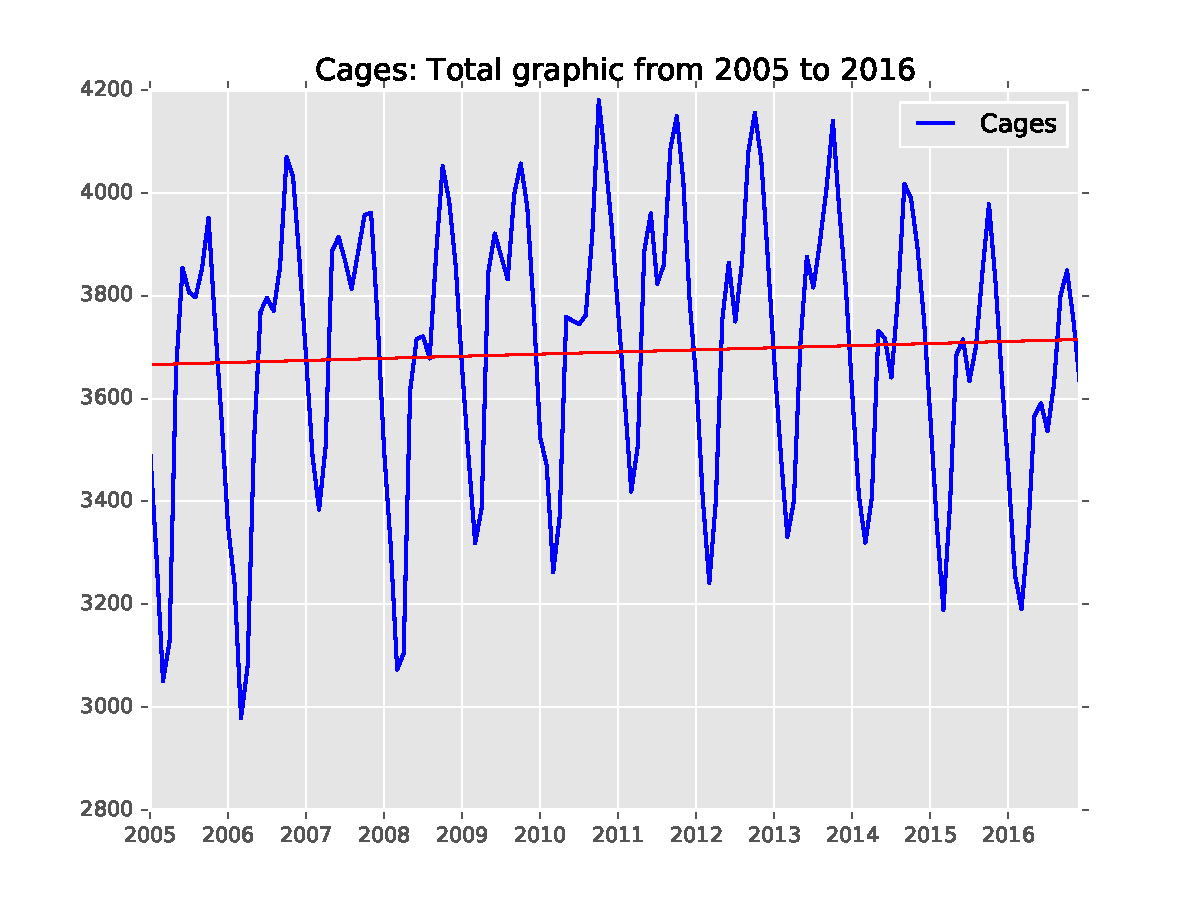
\includegraphics[width=1\textwidth]{Files/Cages_Total.pdf}
    
\end{subfigure}%
\begin{subfigure}{.5\textwidth}
	\centering
    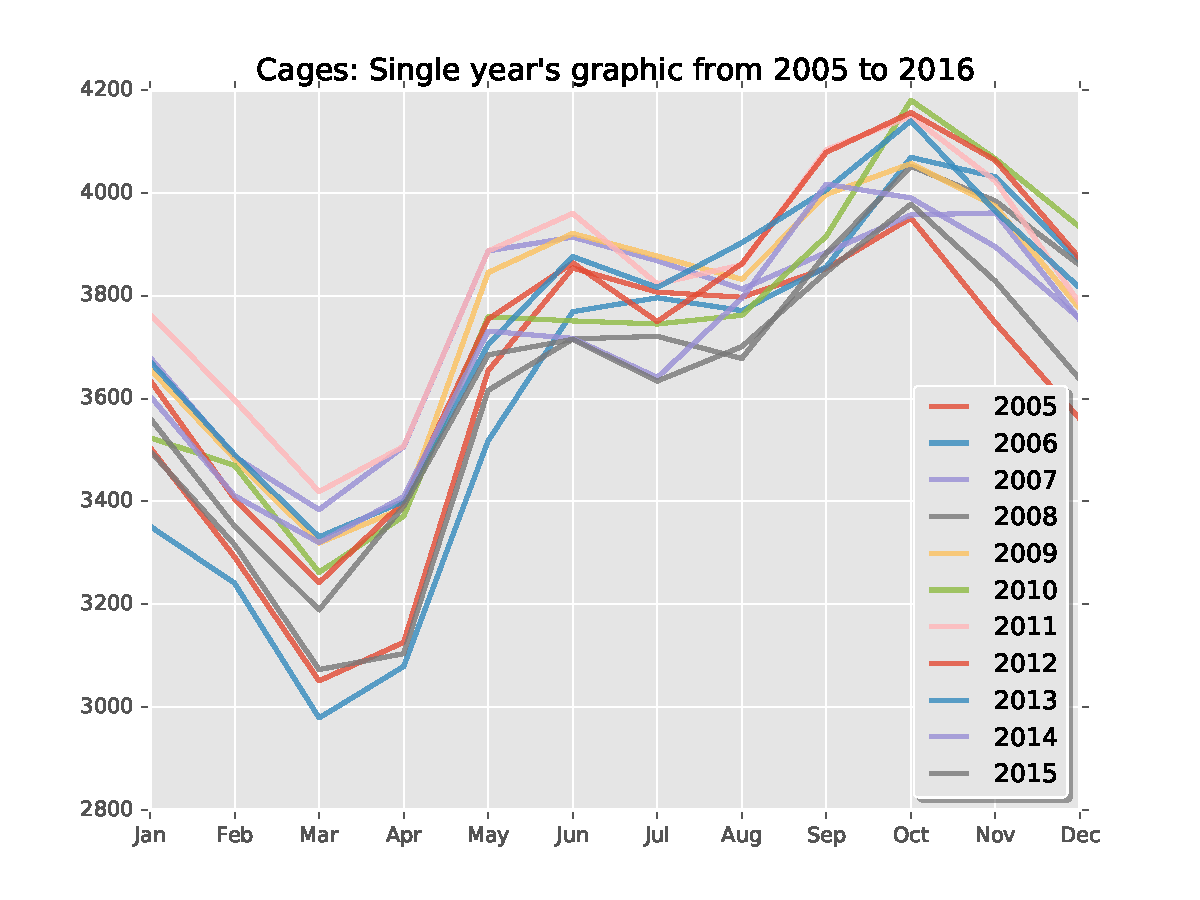
\includegraphics[width=1\textwidth]{Files/Cages_Years.pdf}
\end{subfigure}%
\end{figure} 

\begin{figure}[H]
\begin{subfigure}{.5\textwidth}
	\centering
    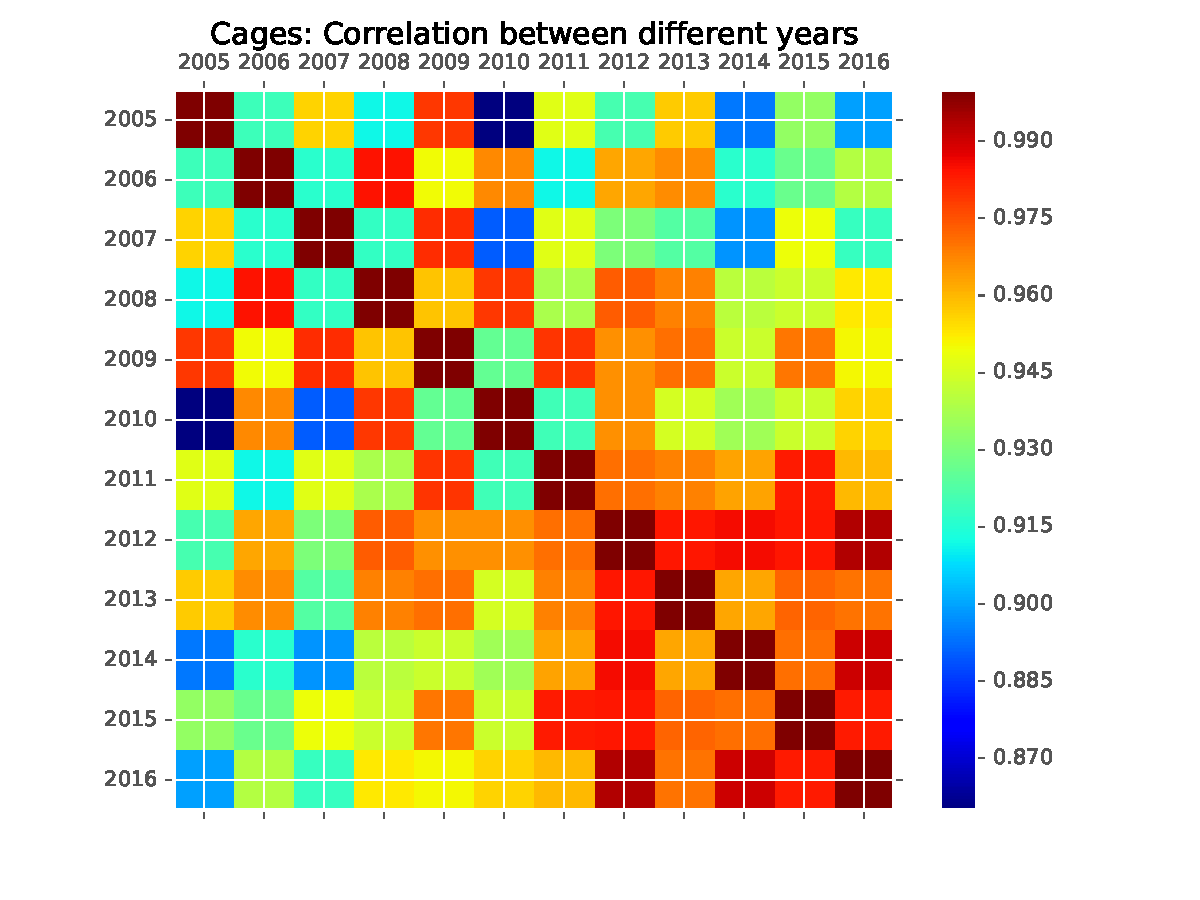
\includegraphics[width=1\textwidth]{Files/Cages_Years_Matrix.pdf}
\end{subfigure}%
\begin{subfigure}{.5\textwidth}
	\centering
    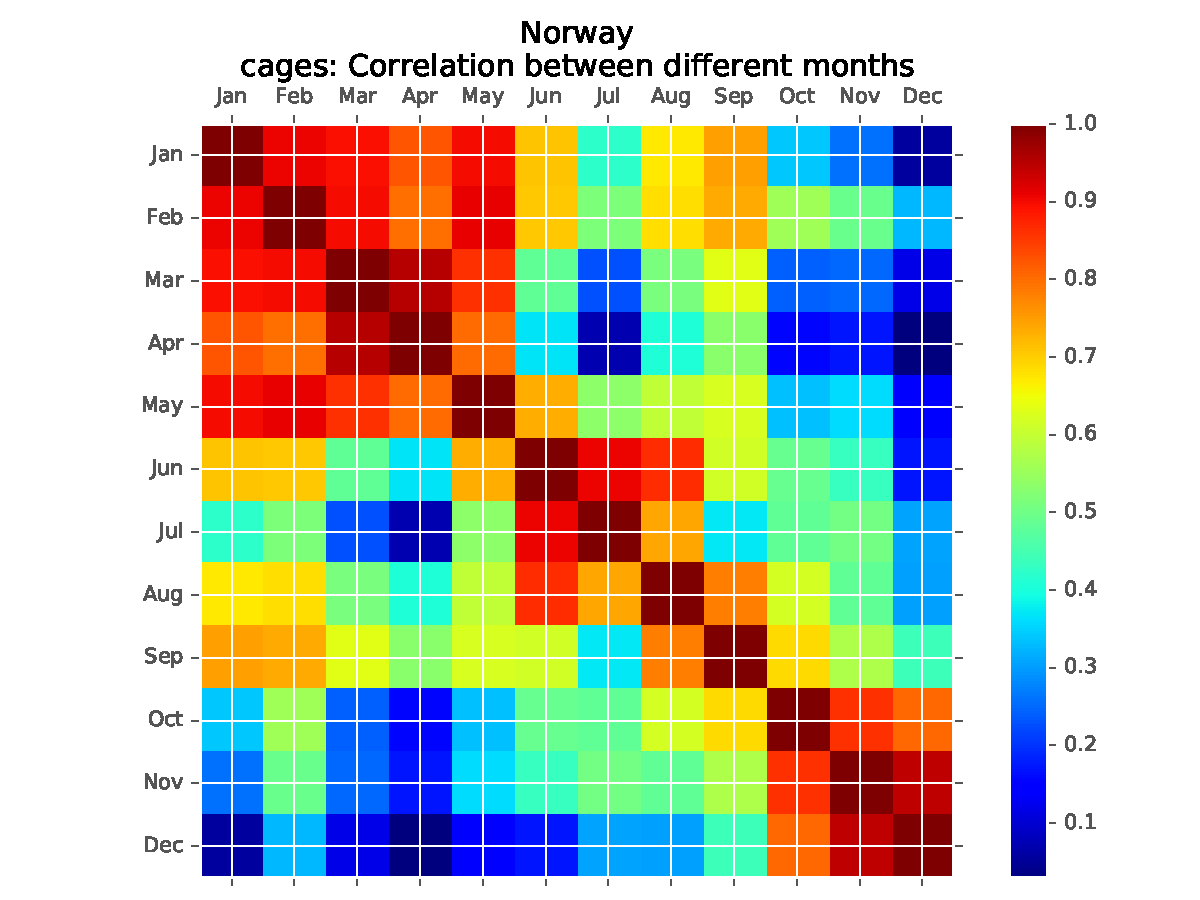
\includegraphics[width=1\textwidth]{Files/Cages_Months_Matrix.pdf}
\end{subfigure}%
\end{figure}

\newpage

\section{Multiple Inputs Analyzer}
The implementation of this Analyzer can be divided in the following parts:
\begin{itemize}
\item MIA imported libraries. 
\item MIA part I: Calculate the correlation coefficients between the different input of a dataset, save the result and display it in a matrix.
\item MIA part II: Display the comparison graphic between the different input's trend line normalized angular coefficients.
\end{itemize}

It's possible to check out the total implementation of the MIA in the appendice  [\ref{MIA_Implementation}].

\subsection{MIA: Imported libraries}
Specific Python libraries have been imported for the implementation of this system.
It's possible to find out a list of this libraries with a specific description for each of them in the appendice [\ref{MIA_Libraries}].

\newpage

\subsection{MIA section I: Total Correlation Coefficients}
\textbf{Goal:}\\
Calculate and save the correlation coefficients between different inputs of the current dataset and then show it with a matrix.

\textbf{Requirements:}\\
To let the MIA system works in a proper way, is necessary that the current dataset has been already analyzed from the SIA system.

\textbf{Implementation:}\\
To reach the current goal have been used the scientific computing library "numpy", that allows to calculate the correlation coefficients between data. Then the library "pyplot" has been used to display the results on a matrix.
\begin{lstlisting}
numpy.corrcoef()
figure = pyplot.figure()
ax = figure.add_subplot()
ax.matshow()
\end{lstlisting}

It's possible to check out the full ccommented code in the appendice: [\ref{MIA_section_I}]

\textbf{Results:} \\
This part of the MIA implementation allows to calculate the correlation coefficients value between each single inputs and then also to display and save it. It looks like:

\begin{figure}[H]
	\centering
    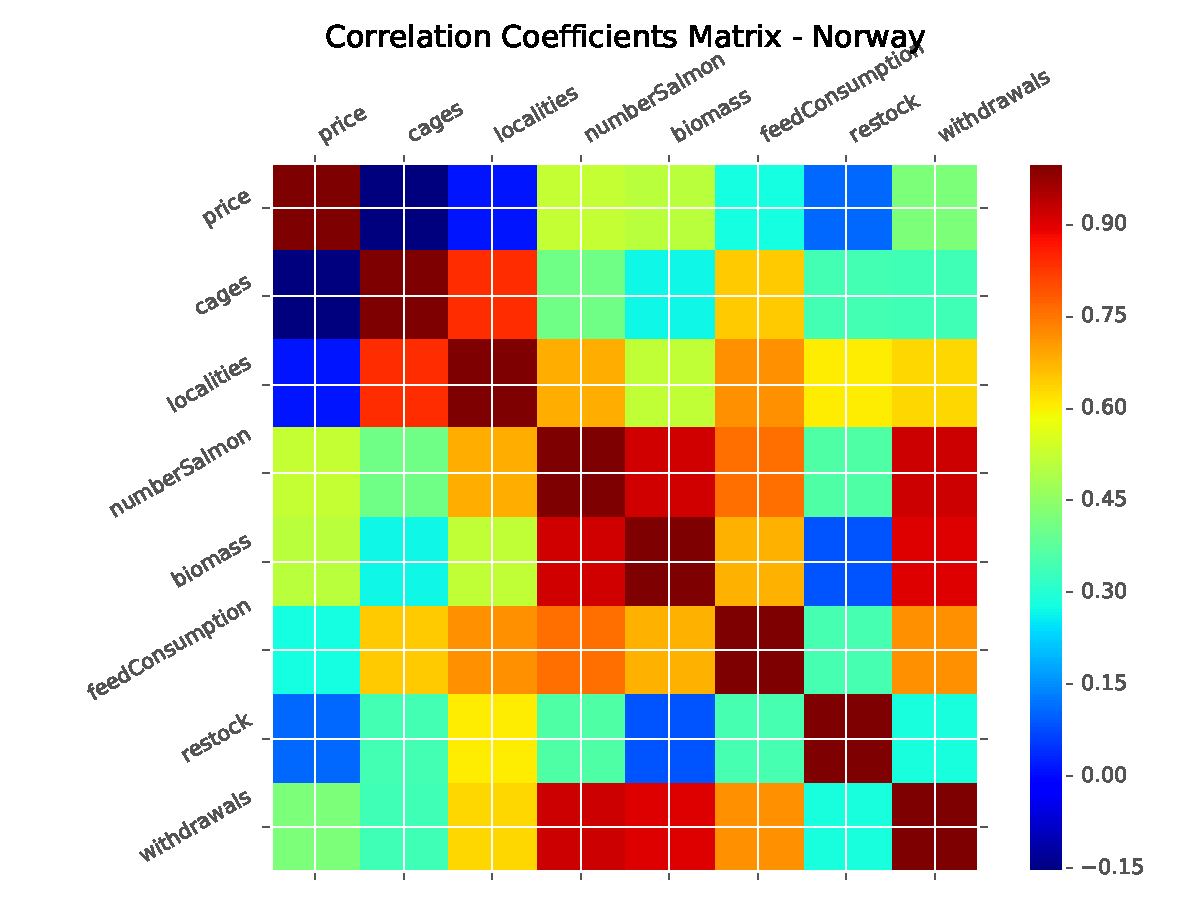
\includegraphics[width=0.85\textwidth]{Files/Total_Dataset_Matrix.pdf}
    \caption{Correlation matrix between different inputs with data.}
\end{figure}

\subsection{MIA section II: Normalized Angular Coefficients}
\textbf{Goal:}\\
Display the comparison graphic between the normalized angular coefficient of each input trend line.

\textbf{Requirements:}\\
To let the MIA system works in a proper way, is necessary that the current dataset has been already analyzed from the SIA system.

\textbf{Implementation:}\\
Also to reach this goal have been used the two libraries "pandas" and "pyplot". The first one allows us to read the values that the library "pyplot" will display, in this case in a histogram.
\begin{lstlisting}
pandas.read_csv()
pyplot.barh()
\end{lstlisting}

It's possible to check out the full ccommented code in the appendice: [\ref{MIA_section_II}]

\textbf{Results:} \\
This part of the MIA implementation allows to display a graphic that compare the normalized angular coefficients for each single input that have been already calculated and reported in a document. The result graphic look like:

\begin{figure}[H]
	\centering
    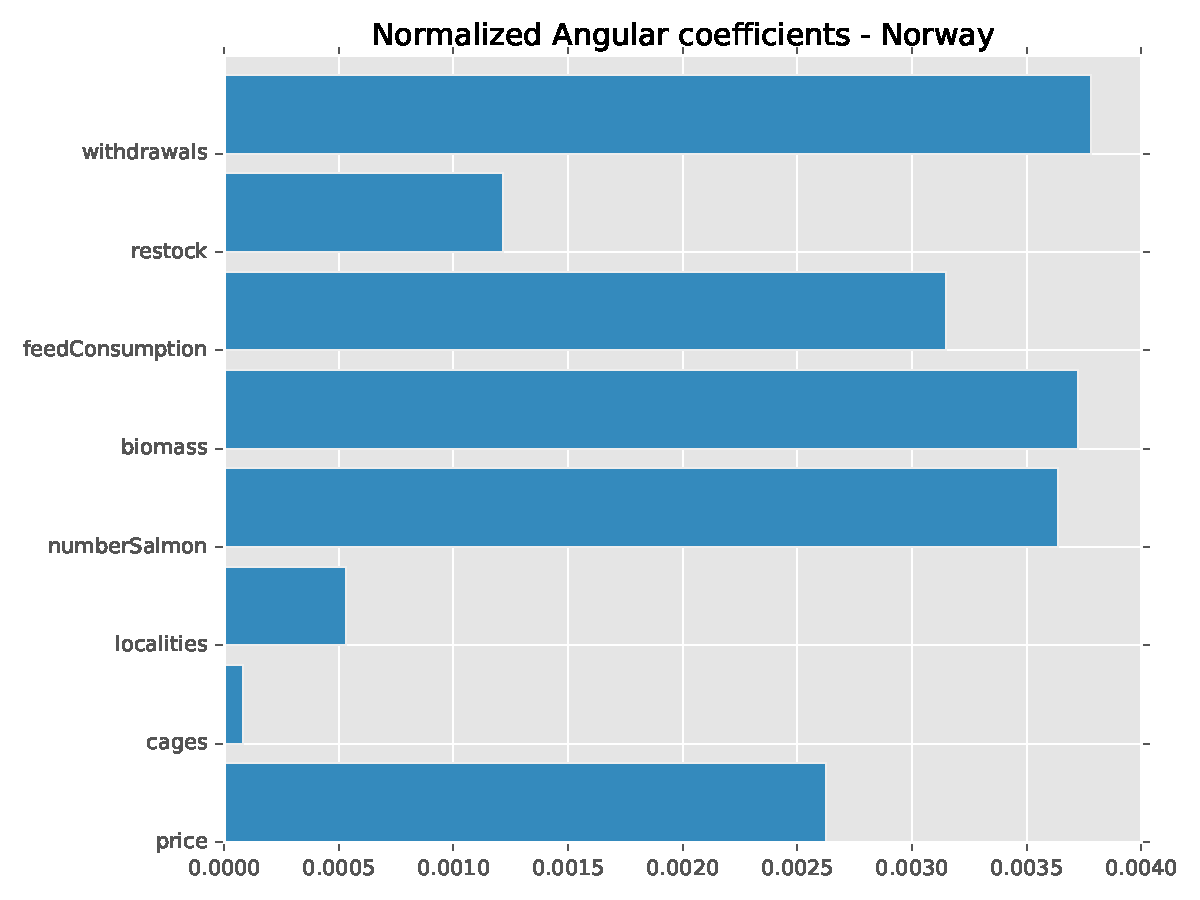
\includegraphics[width=0.90\textwidth]{Files/Norm_Ang_Coeffs.pdf}
    \caption{Normalized angular coefficients of each input's trendline.}
\end{figure}


\newpage

\section{Data Displaying: Map graphic}
\textbf{Goal:}\\
The main goal of this phase is to display the county data values in a easy way to understand and analyze.\\
In this particular case would be useful to display it on a real map of Norway, in order to be able to have an overview about all the counties about different parameters.

\textbf{Requirements:}\\
One parameter in input which has a single value for each county.

\textbf{Implementation:}\\
The library "shpreader" allows to read the extension file ".shp", which in this particular case contains the Norway's shape.\\
Then we can display the current shape using the "pyplot" library and set the colors based on the input values with the library "matplotlib".\\

\begin{lstlisting}
shpreader.Reader().geometries()

plt.figure()
ax = plt.axes()
axes.add_geometries

plt.get_cmap
matplotlib.colors.Normalize
\end{lstlisting}


\textbf{Results:} \\

\begin{figure}[H]
    	\makebox[\textwidth][c]{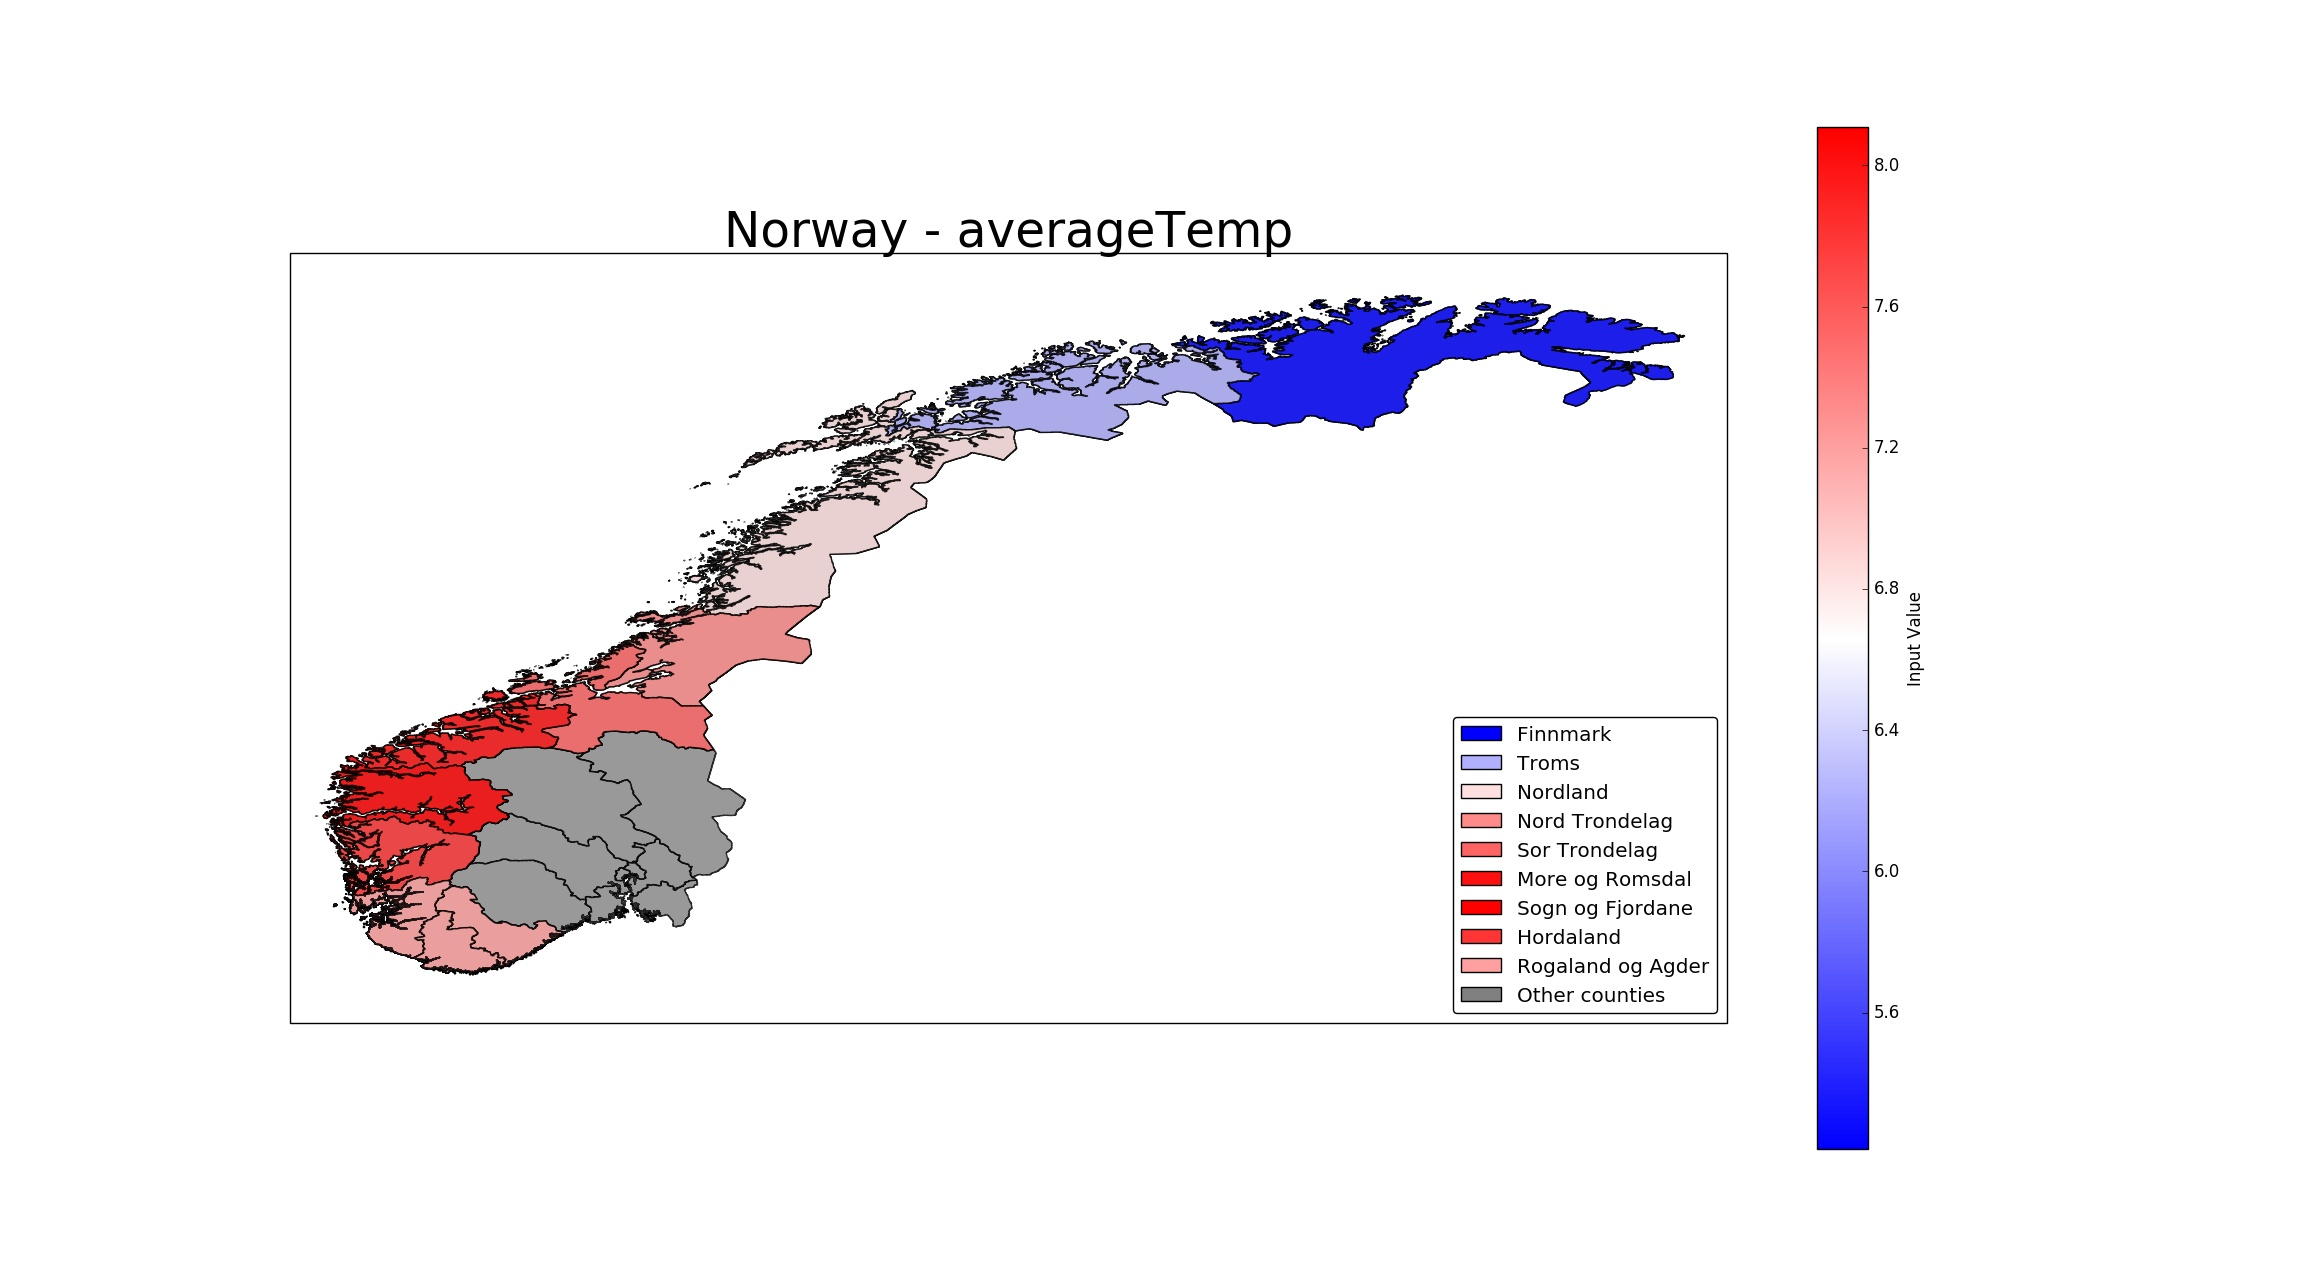
\includegraphics[trim={0cm 2cm 0 3cm},clip, width=0.8\textwidth]{Files/Norway-averageTemp.jpeg}}
    \caption{Average Sea Temperature from 2007 to 2014 in Norway.}
\end{figure}

\newpage

\section{Extract information from data}



\chapter{Prediction of values}

Some basic and general goals were defined before starting this phase, with the idea of "doing more if it's possible". Basically the main purpose was the one of, after the previous analysis, predict some values and evaluate the quality of the results.
This prediction system was not defined with some specific requirements, so the first main problem was to find a reliable, accurated and user-friendly way to predict and display prediction of values.

Since the current dataset can be considered like a time series, in this phase we will develop the data prediction system using an ARIMA machine implemented in python.

The ARIMA machine can be configured with several configurations, it allows you to have more accurated results; so the first thing was to find the right configuration of the ARIMA machine of each single input which we are interested to forecast.

During this phase of the work have been implemented 3 different subsystems for different purposes:
\begin{enumerate}
\item Evaluating System
\item Training System
\item Future Prediction System
\end{enumerate}

\newpage 

\section{Requirements for reusability}
The subsystems implemented during this phase of the work are almost completely reusable.\\
The reusability this systems allows to get some prediction of values about different kind of dataset, in particular:
\begin{itemize}
\item The "Evaluating System" is actually 100\% reusable, and you can use it for evaluate any kind of dataset.
\item The "Future Prediction System" is completely reusable as well, you should only modify the historic values and the real values inside the dataset for it works in a proper way.
\item The "Training System" has been implemented for testing the current dataset, so it's not completely reusable but could be changed very easily and let it works also for other data input.
\end{itemize}

\newpage
\section{Evaluating System}
\textbf{Goal:}\\ 
Used for evaluate different configurations of ARIMA machine. \\ 
It tests 112 different configurations for each single input that we would like to forecast and report the results with each MAPE (Mean Average Percentage Error) values.

\textbf{Requirements:}\\
There are not strict requirements needed. There are no type of restriction neither about the length or about the type of data.

\textbf{Code implementation:}\\
The most important part of the code about the Evaluating System is the following.\\
Basically the method ARIMA() allows to train a model based on historic values (history) and a specific order (p,d,q). After that it's possible to call the method forecast() through the trained model and having some predictions like result.
\begin{lstlisting}
model = ARIMA(history, order=arima_order)
model_fit = model.fit(disp=0)
yhat = model_fit.forecast()[0]
\end{lstlisting}

This system will provide 112 different ARIMA configurations results for each single input, and in particular it will display the best ARIMA configuration, that is the one with the lower MAPE.

\textbf{Results:}\\
The system will display the MAPE between real value and predicted values for each single tested ARIMA machine, in particular the configuration that gives the best result.
All these results have been reported in a document and then also displayed with a 3D graphic that allows to see the MAPE value for each different order in input.

\begin{figure}[H]
	\raggedleft
	\makebox[\textwidth][c]{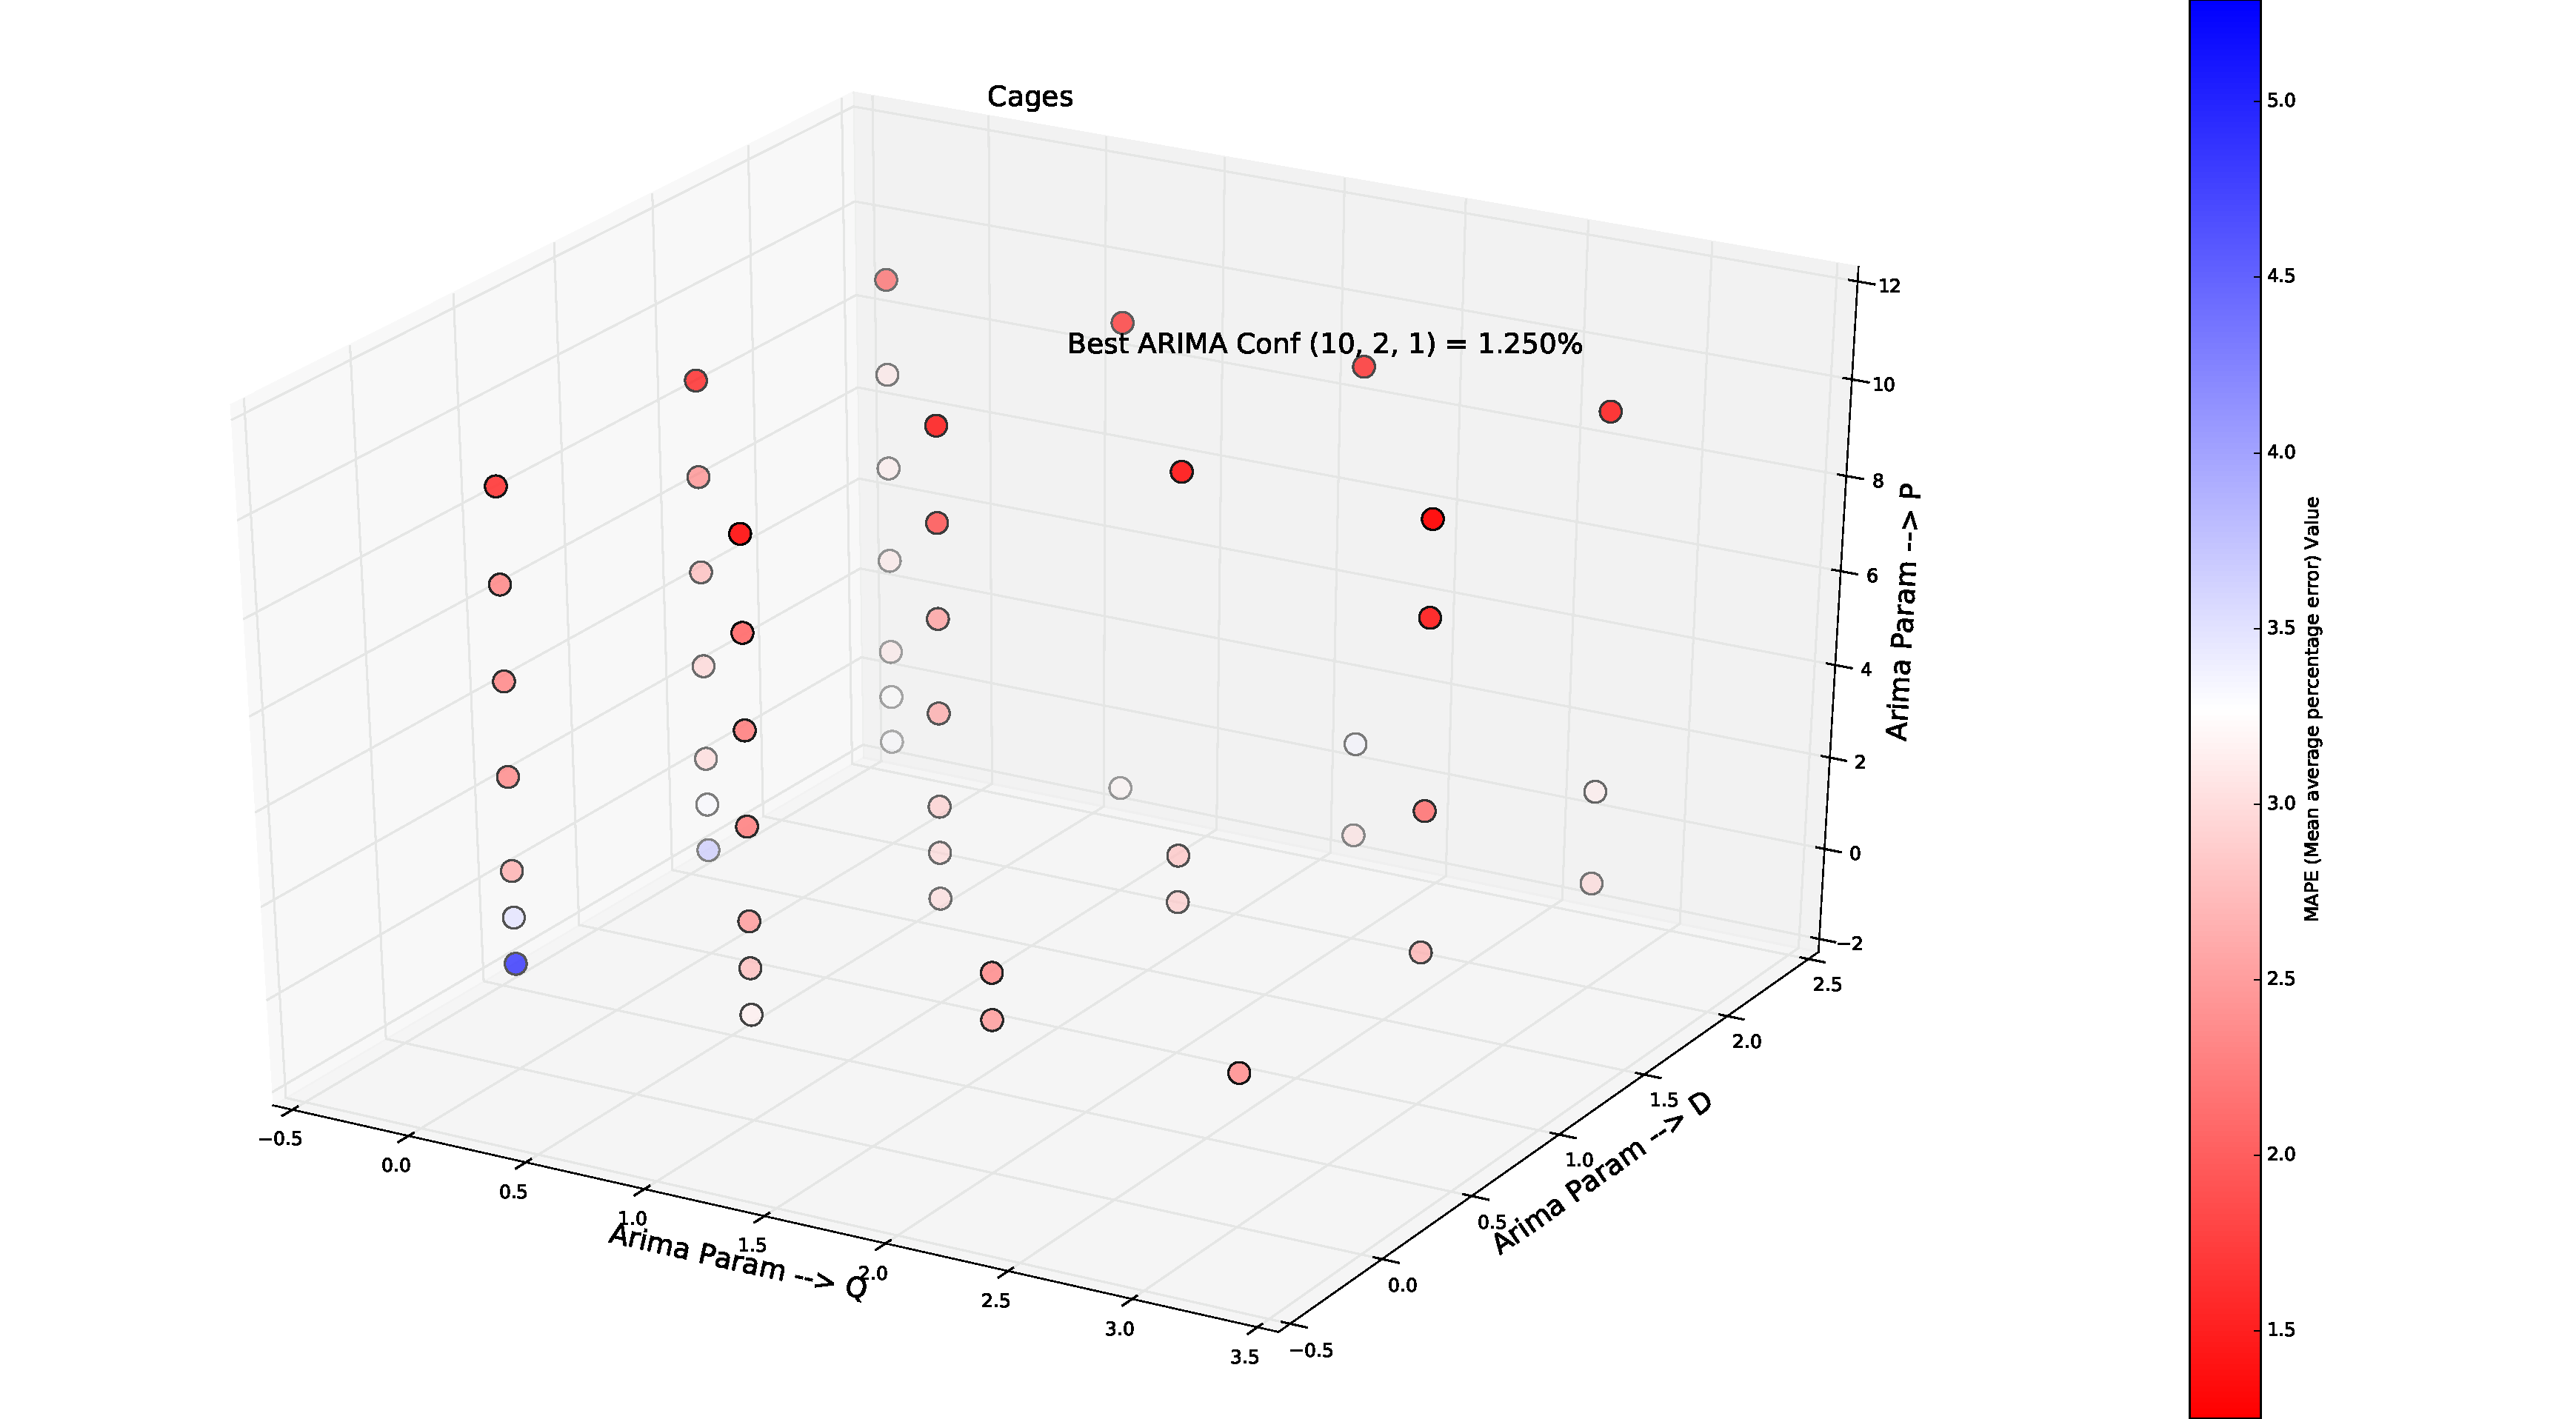
\includegraphics[width=0.6\textwidth]{Files/Cages_MAPE.pdf}}
    \caption{Graphic that displays different MAPE values for each ARIMA order.}
\end{figure}

 
 
\newpage
\section{Training System}
\textbf{Goal:}\\ 
This system has the goal of training/testing a specific ARIMA configuration on a particular data input, and see how much accurate it is. 

\textbf{Requirements:}\\
Since this Traning System has been used mainly for train and test the current dataset, it need to have like input a dataset that follows the same format:\\
- Data content: 144 values, 1 value for each month from 2005 to 2016

\textbf{Code implementation:}\\
First of all this system it's going to split the input data in two part:\\
- Train data: values which the ARIMA model is going to use for training. \\
- Test data: values which are hided by the forecasting model. \\
Once the ARIMA model has been created, the system will try to predict the future values, that are actually the "Test data".\\

\begin{lstlisting}
model = ARIMA(history, order=arima_order)
model_fit = model.fit(disp=0)
yhat = model_fit.forecast()[0]
\end{lstlisting}

Once the predictions have been calculated it's possible to display the "Test data" (that are the real values) and the predicted values, just to see how much the ARIMA configuration is accurate.

\begin{lstlisting}
series = pd.read_csv("Dataset.csv", usecols=[sys.argv[1]])
series.plot(color="blue", linewidth=1.5,
		 label="Series: "+sys.argv[1])


output = Series.from_csv('Output_Files/predictions.csv')
output.plot(color="red", linewidth=1.5,
		label="Prediction test:")
\end{lstlisting}

\newpage

\textbf{Results:}\\
The following picture is an output example of this training system. \\
It actually allows to have an idea about how accurate is that ARIMA configuration for predictions.
\begin{figure}[H]
	\centering
    \makebox[\textwidth][c]{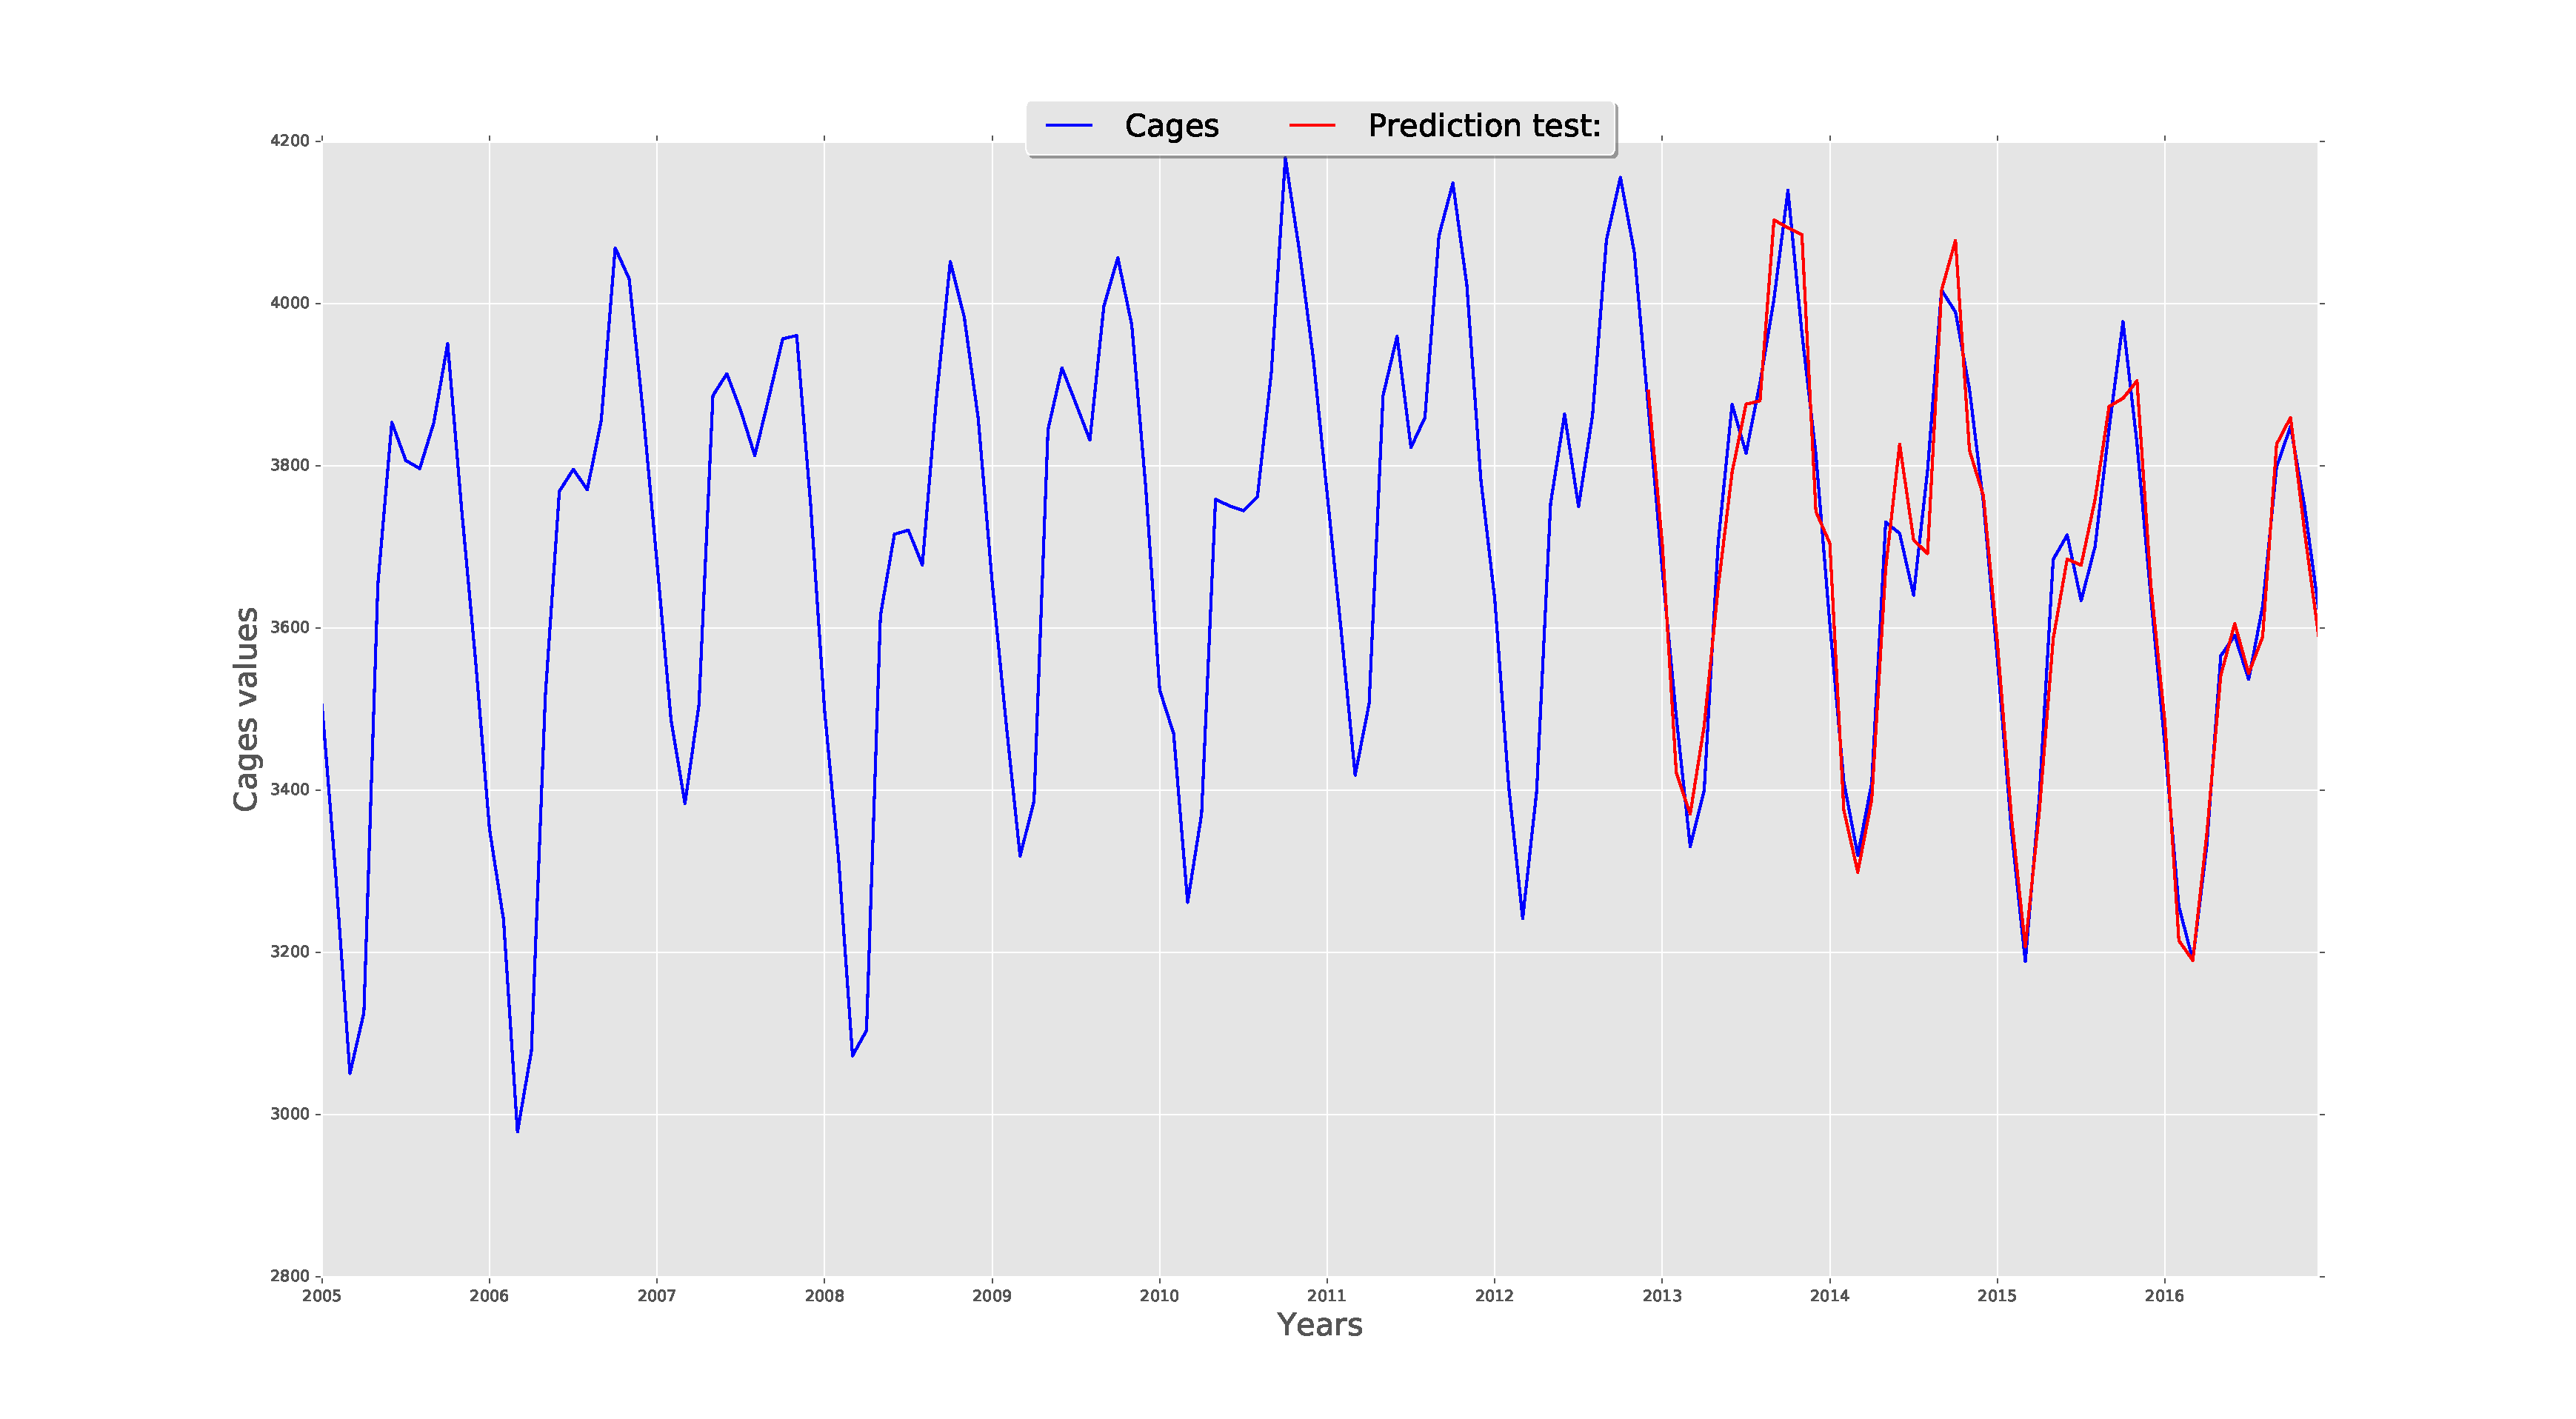
\includegraphics[width=1.5\textwidth]{Files/Cages_TRAIN.pdf}}
    \caption{Graphic that displays the predicted values from a particular ARIMA machine configuration and the historic real values.}
\end{figure}


\newpage
\section{Future Prediction System}
\textbf{Goal:}\\ 
This part of the work has the goal of display some real prediction of values in the future. \\
It basically collects real future values, in this particular are values about 2017, of each single input and then, once calculated also the prediction values, it's going to display on the same graphic:\\
- Historic values\\
- Predicted future values\\
- Real values (if are available)

\textbf{Requirements:}\\
This system has to be as much reusable as possible, so there are not that strict requirements. You can reuse this Future Prediction System with any kind of dataset with no restrictions about length. \\
The only requirement to let it works in a proper way is that you have to set the historic and real values datasets in the right way; it means that you have to write down the historic values in the dataset in this way:


\begin{table}[ht] 
    \centering 
    \begin{tabular}{ | l | l | l | p{5cm} |}
        \hline
        Index 	& Input1 	& Input2			\\ \hline
          	1 	& Value1 	& Value1			\\ \hline
          	2 	& Value2 	& Value2			\\ \hline
          	3 	& Value3	& Value3 		\\ \hline
          	... & ... 		& ...				\\ \hline
           	120 & Value120 & Value120	\\ \hline
          	121 & Value121 & Value121	\\ \hline
 			122 & Value122 & Value122	\\ \hline
    \end{tabular}
    \caption{Historic dataset structure}
    \label{table: pred_historic_values} 
\end{table} 

And then, if you want to compare the predicted values with some real values that are already available, you have to set the real values dataset in this way:


\begin{table}[ht] 
    \centering 
    \begin{tabular}{ | l | l | l | p{5cm} |}
        \hline
        Index & Input1 & Input2 		\\ \hline
          	123 & Value123 & Value123 	\\ \hline
          	124 & Value124 & Value124 	\\ \hline
          	125 & Value125 & Value125 	\\ \hline
          	126 & 	&					\\ \hline
          	127 & 	&					\\ \hline
          	128 & 	&					\\ \hline
 			129 & 	&					\\ \hline
    \end{tabular}
    \caption{Future real values dataset structure}
    \label{table: pred_real_values} 
\end{table} 

\newpage
\textbf{Code implementation:}\\
First of all a new ARIMA model it's created using the current historic values and a specific ARIMA-Order, that it should be the Best ARIMA-Order calculated during by the Evaluation System.\\
Then, once the model is ready, it's possible to calculate as many prediction values in the future as you want. \\
\begin{lstlisting}
model = ARIMA(history, order=arima_order)
model_fit = model.fit(disp=0)
yhat = model_fit.forecast()[0]
\end{lstlisting}

Once the predictions have been calculated, it's possible to display a graphic that contains the historic values, the future predictions value and the real future values (if already available).
\begin{lstlisting}
# 1) Historic values
series = pd.read_csv("HISTORIC DATASET", 
			usecols=[sys.argv[1]])
series.plot(color="blue",linewidth=1.5)

# 2) Predicted future values
series = Series.from_csv("PREDICTIONS DATASET")
series.plot(color="red", linewidth=1.5, 
			label="Prediction Results")

# 3) Real future values
series = pd.read_csv("REAL VALUES DATASET")
pyplot.plot(series["Index"], series[sys.argv[1]],
	color="green", linewidth=1.5, label="Real values")

\end{lstlisting}

\newpage 

\textbf{Results:}\\
The system implemented during this phase allows to predict future for as many months as you want in the future and to display it, compared also with the historic values and real values once are available. The output graphic look like:
\begin{figure}[H]
	\centering
    \makebox[\textwidth][c]{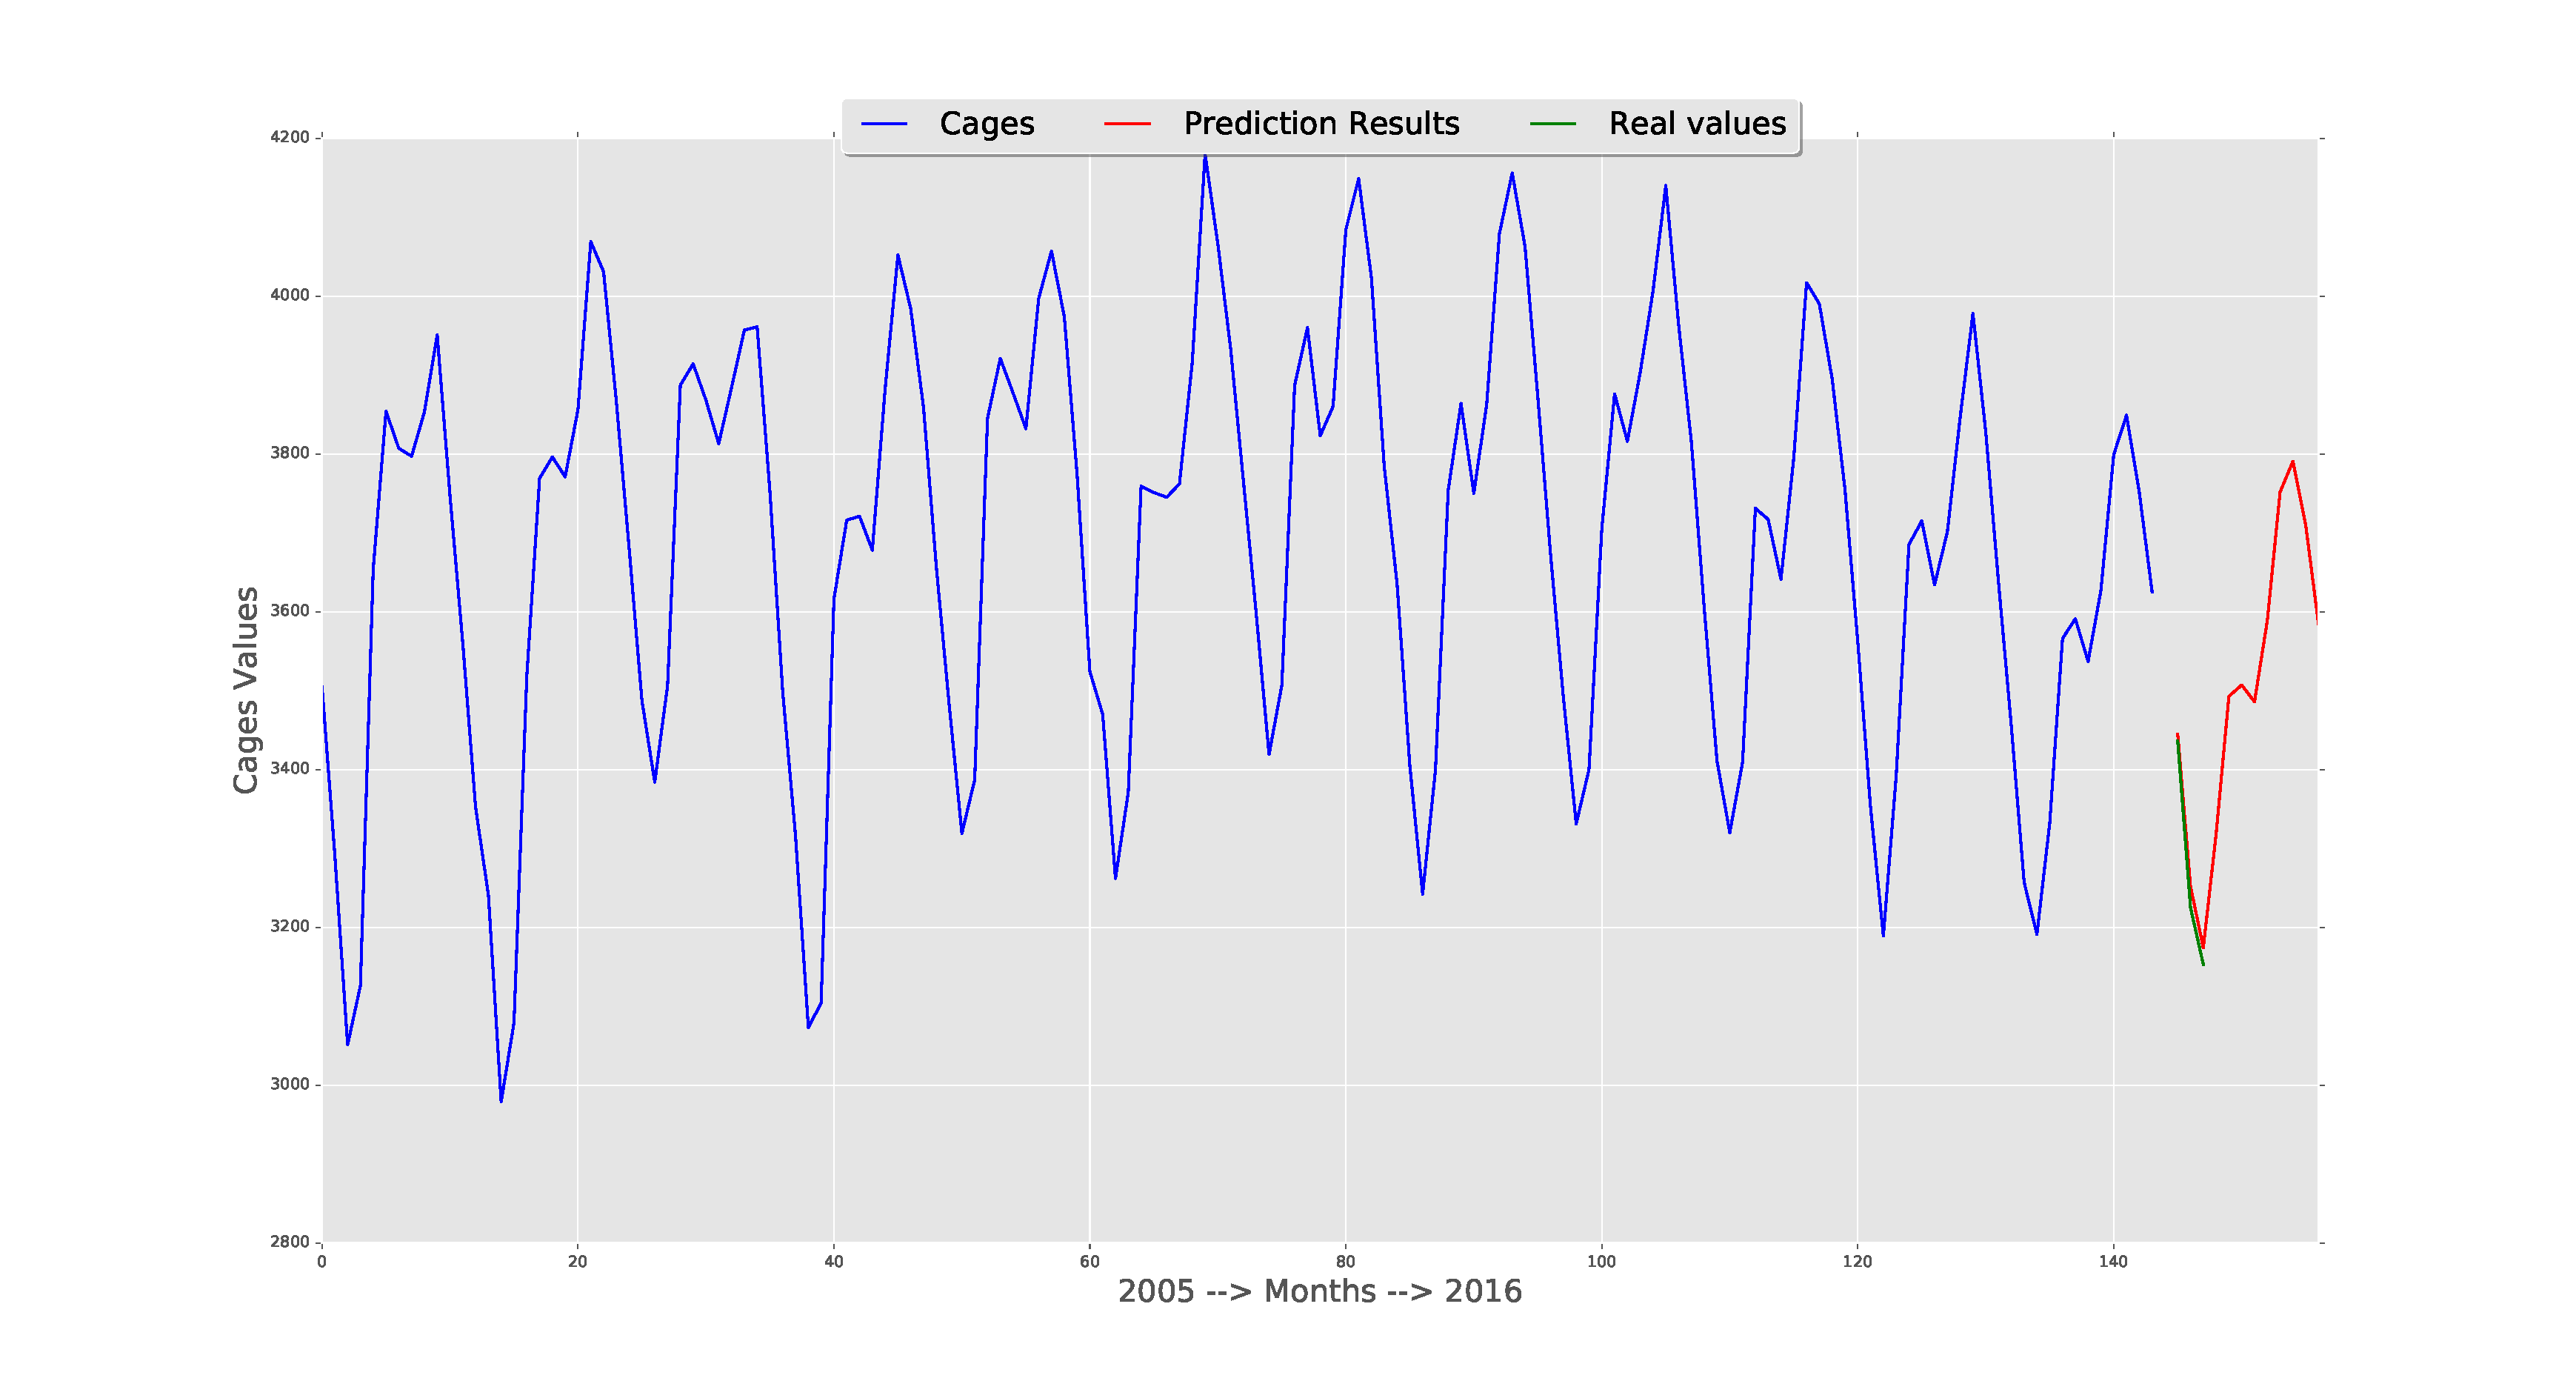
\includegraphics[width=1.5\textwidth]{Files/Cages_Predictions.pdf}}
    \caption{Graphic that display historic, future and predicted values of a input.}
\end{figure}

\newpage







\chap{Results}

The main result of this work is the implemented "Python Analyzer System" itself. It actually provides an automatic way to make an initial analysis and display the results of any input dataset.

Further more has been provided an initial Python implementation of:
\begin{itemize}
\item Future Prediction System
\item Country Map Displaying System
\end{itemize}
\newpage

\begin{figure}[H]
	\centering
    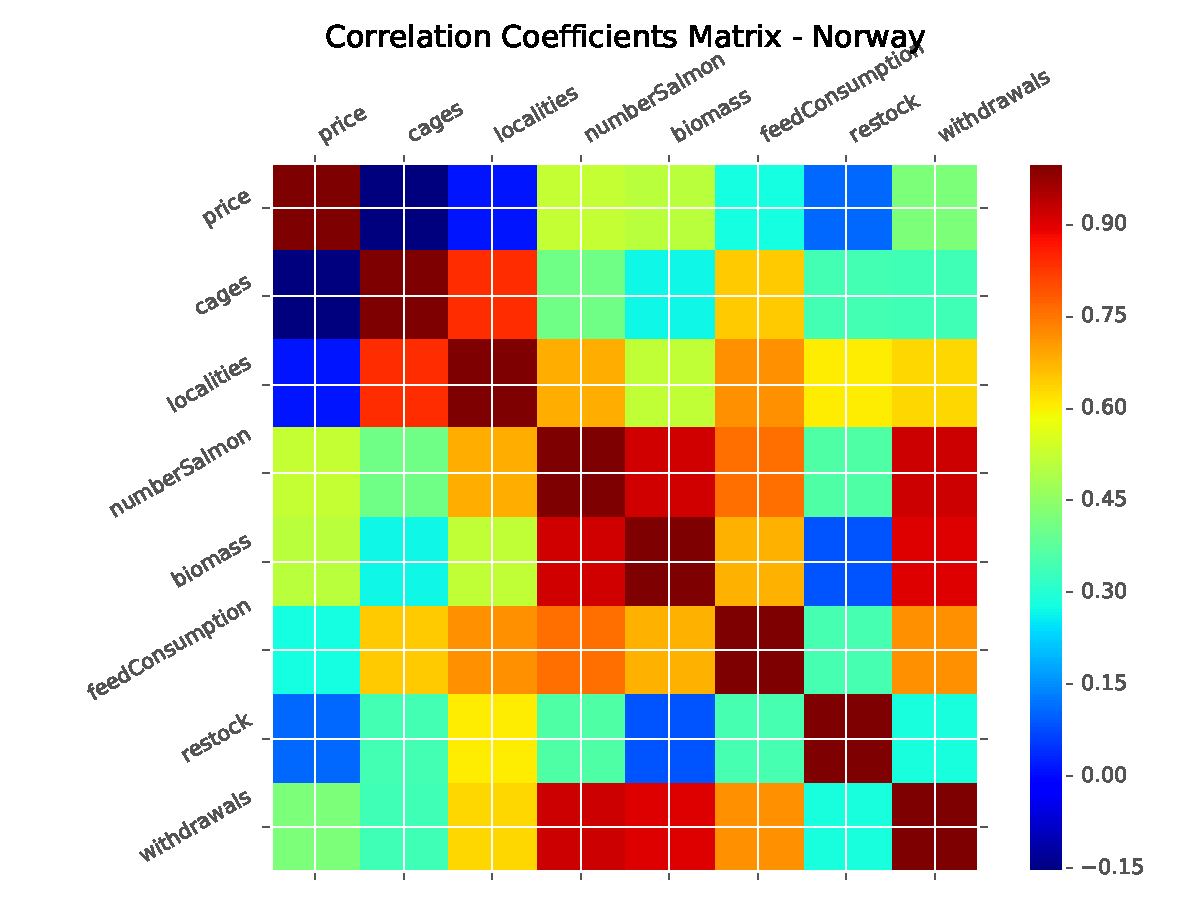
\includegraphics[width=1\textwidth]{Files/Total_Dataset_Matrix.pdf}
    \caption{Correlation matrix between different inputs with data from 2005 to 2016.}
\end{figure}

\begin{table}[ht] 
\makebox[\textwidth][c] {
\resizebox{1.2\textwidth}{!}{\begin{tabular}{ | l | l | l | l | l | l | l | l | l |}
        \hline
INPUTS	& Price 		& Cages 			& Localities		& numberSalmon 		& biomass 		& feedConsumption 		& restock 		& withdrawals 				\\ \hline
Price			& 1			& -0.16		& 0.02 		& 0.52		& 0.51		& 0.28		& 0.11 		& 0.43		\\ \hline
Cages			& -0.16		& 1			& 0.84		& 0.41		& 0.27		& 0.64		& 0.34		& 0.34		\\ \hline
Localities		& 0.02		& 0.84		& 1			& 0.68		& 0.52		& 0.72		& 0.6		& 0.63		\\ \hline
numberSalmon	& 0.52		& 0.41		& 0.68		& 1 		& 0.92		& 0.76		& 0.36		& 0.92		\\ \hline
biomass			& 0.51		& 0.27		& 0.52		& 0.92		& 1			& 0.68		& 0.09		& 0.91		\\ \hline
feedConsumption	& 0.28		& 0.64		& 0.72		& 0.76		& 0.68		& 1			& 0.35		& 0.72		\\ \hline
restock			& 0.11		& 0.34		& 0.6		& 0.36		& 0.09		& 0.35		& 1 		& 0.28		\\ \hline
withdrawals		& 0.43		& 0.34		& 0.63		& 0.92		& 0.91		& 0.72		& 0.28		& 1			\\ \hline
    \end{tabular}}}
    \caption{Dataset inputs correlation coefficients value.}
    \label{table: trendline} 
\end{table}

\newpage

\begin{figure}[H]
	\centering
    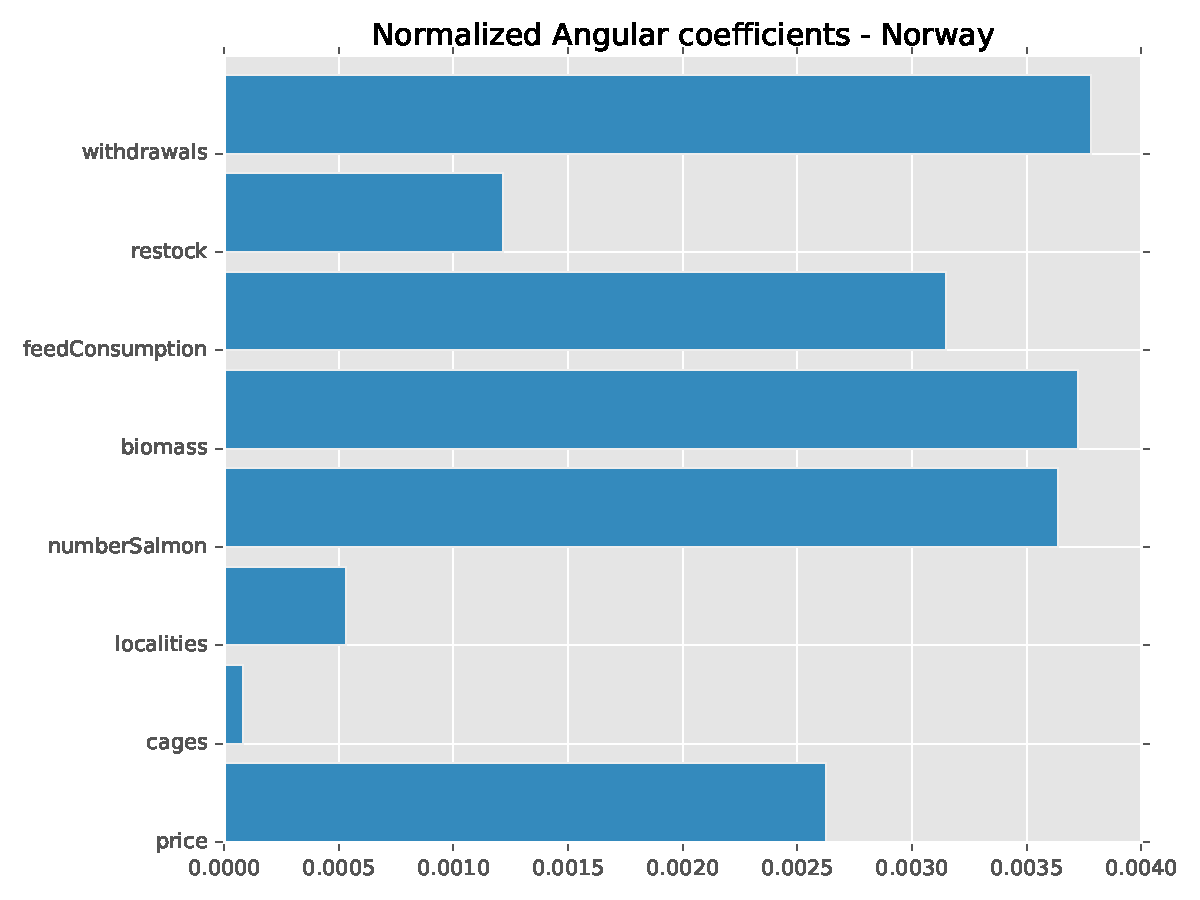
\includegraphics[width=1\textwidth]{Files/Norm_Ang_Coeffs.pdf}
    \caption{Normalized angular coefficients of each input's trendline.}
\end{figure}

\begin{table}[ht] 
	\centering
    \begin{tabular}{ | l | l | l | p{5cm} |}
        \hline
        Input 								& Equation 							& Coeff			\\ \hline
          	Salmon\_withdrawals 			& y=464.755139x+(46295.729945) 		& 464.755139 	\\ \hline
          	Salmon\_biomass\_end\_month 	& y=2832.712270x+(354138.727889) 	& 2832.71227 	\\ \hline
          	Salmon\_number\_end\_month 		& y=1543.298421x+(205325.455772)	& 1543.298421 	\\ \hline
          	Salmon\_consumption\_of\_feed 	& y=620.070855x+(58330.012273) 		& 620.070855	\\ \hline
           	Salmon\_price 			& y=0.178175x+(22.643654)			& 0.1781753878 		\\ \hline
          	Salmon\_restock 				& y=89.230600x+(13390.363406)		& 89.2306 		\\ \hline
 			Localities 						& y=0.343533x+(539.979023) 			& 0.343533		\\ \hline
  			Cages 							& y=0.342834x+(3665.904023) 		& 0.342834 		\\ \hline
    \end{tabular} 
    \caption{Dataset inputs trendline equation}
    \label{table: trendline} 
\end{table}
\begin{table}[ht] 
	\centering
    \begin{tabular}{ | l | l | l | p{5cm} |}
        \hline
        Input 							& Normalized equation 	& Norm Ang Coeffs	\\ \hline
          	Salmon\_withdrawals 		& y=0.003782x+(0.376694)& 0.003782			\\ \hline
          	Salmon\_biomass\_end\_month & y=0.003724x+(0.465599)& 0.003724			\\ \hline
          	Salmon\_number\_end\_month 	& y=0.003639x+(0.484184)& 0.003639			\\ \hline
          	Salmon\_consumption\_of\_feed & y=0.003147x+(0.296085)& 0.003147		\\ \hline
           	Salmon\_price 		& y=0.002625x+(0.333633)
& 0.002625			\\ \hline
          	Salmon\_restock 			& y=0.001217x+(0.182583)& 0.001217			\\ \hline
 			Localities 					& y=0.000531x+(0.834589)& 0.000531			\\ \hline
  			Cages 						& y=0.000082x+(0.877011)& 0.000082			\\ \hline
    \end{tabular} 
    \caption{Dataset inputs normalized trendline equation}
    \label{table: norm_trendline} 
\end{table}

\newpage

\begin{figure}[H]
    \makebox[\textwidth][c]{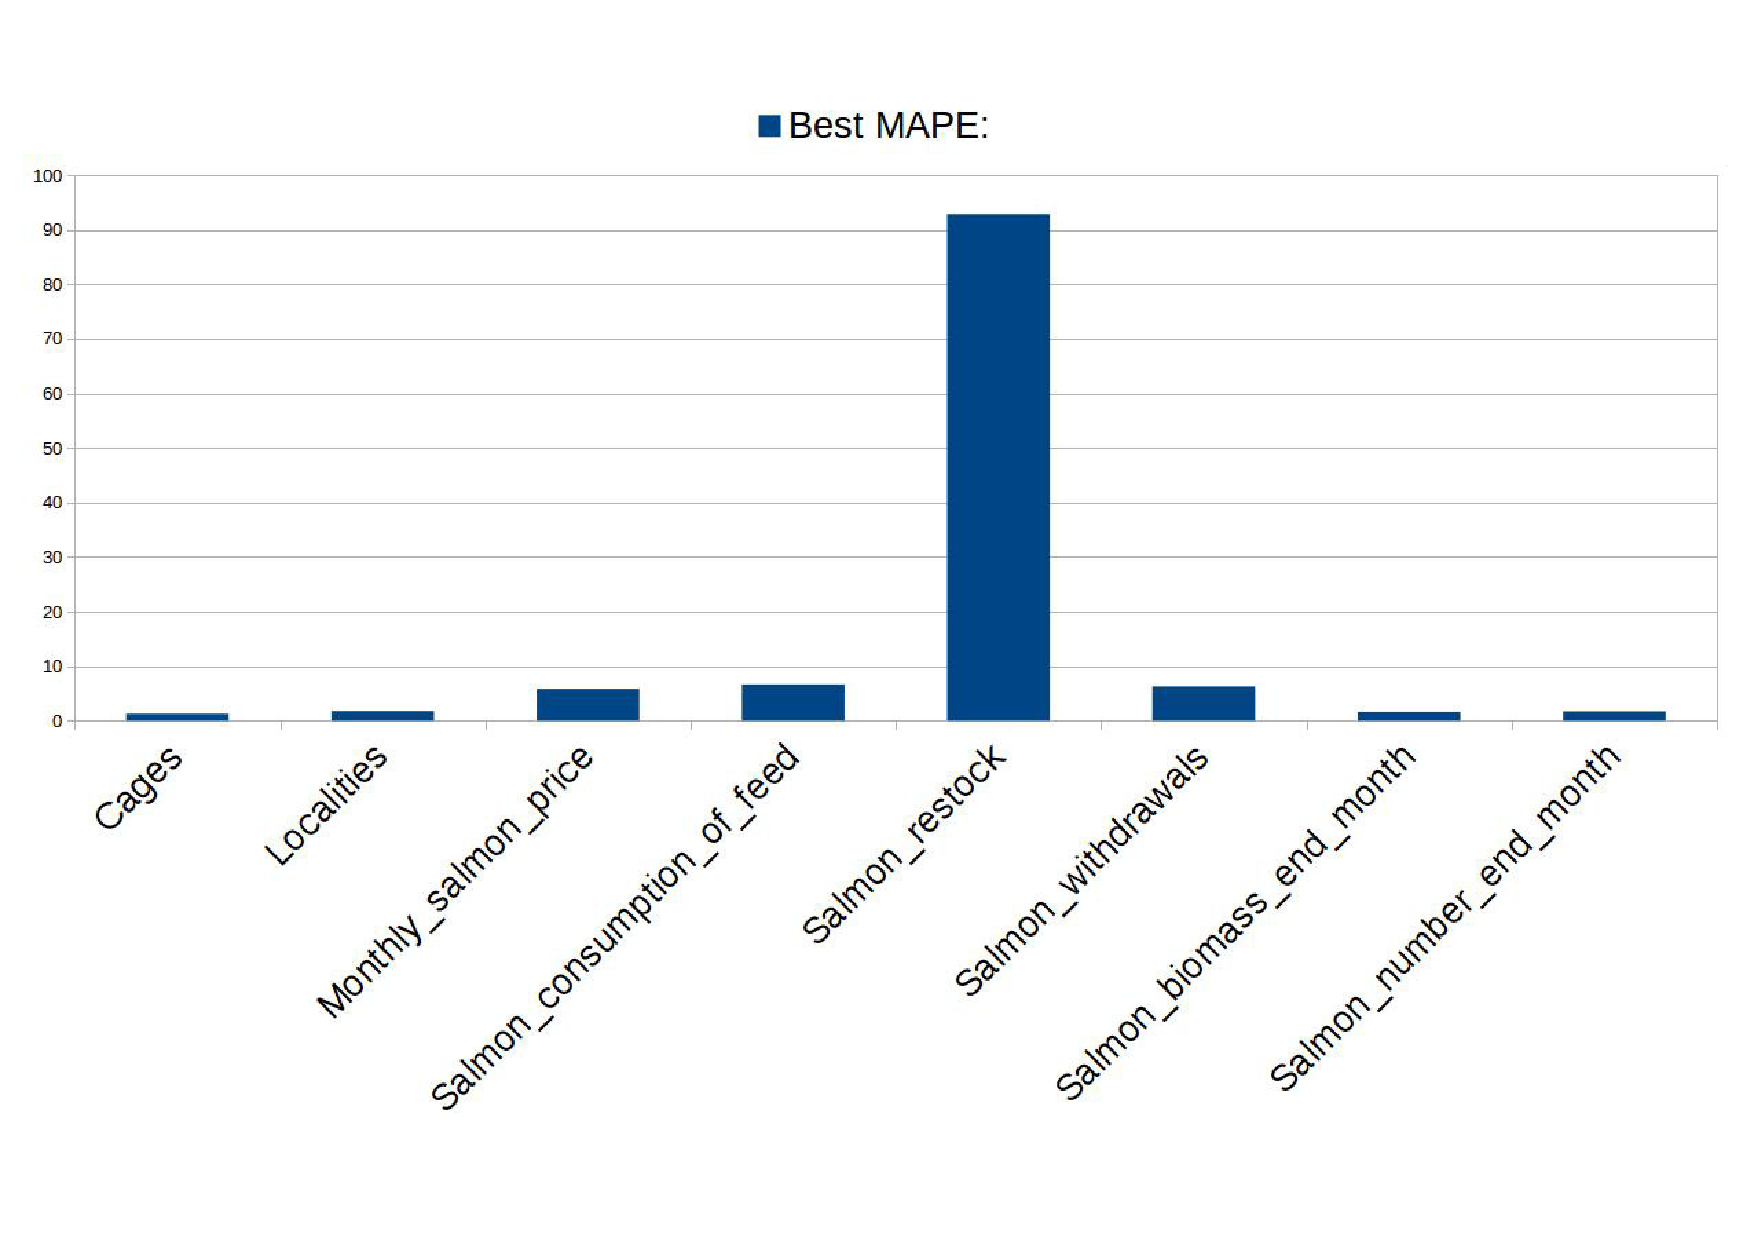
\includegraphics[width=1.2\textwidth]{Files/Best_MAPE.pdf}}
    \caption{Lower MAPE with best ARIMA Configuration for each tested input.}
\end{figure}

\begin{table}[ht] 
	\centering
    \begin{tabular}{ | l | l | l |}
            \hline
Input							&	ARIMA Conf	&	MAPE	\\ \hline
Cages							&	(10,2,1)	&	1.251\%	\\ \hline
Localities						&	(10,0,1)	&	1.779\%	\\ \hline
Salmon\_price 					&	(0,1,1)		&	6.686\%	\\ \hline
Salmon\_consumption\_of\_feed	&	(6,1,0)		&	6.659\%	\\ \hline
Salmon\_restock 				&	(10,0,1)	&	96.006\%	\\ \hline
Salmon\_withdrawals 			&	(10,0,1)	&	6.277\%	\\ \hline
Salmon\_biomass\_end\_month		&	(8,1,0)		&	1.601\%	\\ \hline
Salmon\_number\_end\_month 		&	(10,2,0)	&	1.723\%	\\ \hline
    \end{tabular}  
    \caption{Dataset inputs normalized trendline equation}
    \label{table: Best ARIMA configurations with relative MAPE result in the Evaluation Test} 
\end{table}

\newpage

\makebox[\textwidth][c]{
\resizebox{1.3\textwidth}{!}{
\begin{tabular}{|c|c|c|c|c|c|c|c|c|c|c|c|c|c|}
\hline
\multirow{3}{*}{Months} & \multicolumn{3}{c|}{Cages} & \multicolumn{3}{c|}{Localities} & \multicolumn{3}{c|}{Salmon Biomass} & \multicolumn{3}{c|}{Salmon Number}\\
\cline{2-13}
 & Real & Pred & Error & Real & Pred & Error & Real & Pred & Error & Real & Pred & Error \\
\hline
 January 2017 & 3436 & 3444.87 & 0.26\% & 539.000 & 543.41 & 0.82\% & 738902 & 732841.36 & 0.82\% & 369274 & 366826.189 & 0.66\%\\
\hline
 February 2017 & 3225 & 3251.915 & 0.83\% & 523.000 & 529.05 & 1.16\% & 712981 & 709931.42 & 0.43\% & 347824 & 352905.30 & 1.46\% \\
 \hline
 March 2017 & 3153 & 3164.190 & 0.67\% & 529.000 & 534.29 & 1.00\% & 667749 & 679405.11 & 1.75\% & 343636 & 349747.77 & 1.78\%\\
 \hline
 April 2017 & & 3317.814 & & & 549.14 & & & 657418.41 & & & 369616.83 &  \\
 \hline
 May 2017 & & 3492.701 & & & 550.64 & & & 646850.14 & & & 387244.43 &  \\
 \hline
 June 2017 & & 3507.062 & & & 545.66 & & & 653574.18 & & & 387630.48 & \\
 \hline
 July 2017 & & 3485.804 & & & 560.58 & & & 678469.77 & & & 384314.00 &  \\
 \hline
 August 2017 & & 3588.373 & & & 584.55 & & & 707646.99 & & & 394062.43 & \\
 \hline
 September 2017 & & 3751.633 & & & 596.32 & & & 734628.28 & & & 411164.01 & \\
 \hline
 October 2017 & & 3790.521 & & & 589.11 & & & 757679.66 & & & 411094.09 & \\
 \hline
 November 2017 & & 3710.033 & & & 576.75 & & & 770838.51 & & & 396102.24 & \\
 \hline
 December 2017 & & 3584.505 & & & 563.56 & & & 771279.10 & & & 380399.93 & \\
 \hline
% etc. ...
\end{tabular}  }}


\makebox[\textwidth][c]{
\resizebox{1.3\textwidth}{!}{
\begin{tabular}{|c|c|c|c|c|c|c|c|c|c|c|c|c|c|}
\hline
\multirow{3}{*}{Months} & \multicolumn{3}{c|}{Consumption of feed} & \multicolumn{3}{c|}{Salmon restock} & \multicolumn{3}{c|}{Salmon Withdrawals} & \multicolumn{3}{c|}{Salmon price}\\
\cline{2-13}
 & Real & Pred & Error & Real & Pred & Error & Real & Pred & Error & Real & Pred & Error \\
\hline
 January 2017 & 109341 & 98174.28 & 10.21\% & 4415 & 4734.43 & 7.23\% & 87609 & 90488.98 & 3.29\% & & &\\
\hline
 February 2017 & 88704 & 77998.20 & 12.07\% & 991 & 6904.51 & 596.72\% & 3.29\% & 101295.55 & 11.00\% & & &\\
 \hline
 March 2017 & 87033 & 74726.18 & 14.14\% & 13594 & 15427.63 & 13.49\% & 109498 & 101724.09 & 7.10\% & & &\\
 \hline
 April 2017 & & 88768.11 & & & 39781.36 & & & 95032.95 & & & &\\
 \hline
 May 2017 & & 113280.67 & & & 39438.14 & & & 92065.64 & & & &\\
 \hline
 June 2017 & & 140413.56 & & & 22562.89 & & & 88775.54 & & & &\\
 \hline
 July 2017 & & 164511.15 & & & 20449.85 & & & 92643.44 & & & &\\
 \hline
 August 2017 & & 179690.48 & & & 39487.67 & & & 104102.60 & & & &\\
 \hline
 September 2017 & & 181556.12 & & & 49991.91 & & & 110419.37 & & & &\\
 \hline
 October 2017 & & 169502.10 & & & 31449.69 & & & 107588.69 & & & &\\
 \hline
 November 2017 & & 147770.73 & & & 11698.23 & & & 102943.86 & & & &\\
 \hline
 December 2017 & & 123447.55 & & & 7957.45 & & & 99561.98 & & & &\\
 \hline
% etc. ...
\end{tabular}  }}


 % Results

\chap{Discussion} % Discussion

\chap{Conclusion}

\section{Summary}

\section{Recommendations to future work}

\subsection{Dataset about single locality}
This thesis allows to have a general overview and predictions of values about the aquaculture business in Norway. 

But it would be much more useful, in particular for people into the aquaculture business, to use this system to have an overview and predictions of data provided by a single locality of aquaculture.\\
In this case the system could be used from the owner of the locality to analyze historic values and use the prediction system to have a forecast about some particular parameters.

\subsection{Visualization of the data}

\subsection{Test prediction system with a bigger dataset}

\section{Prediction system as a service}
This system has been developed with the idea that it could become a "Service system", that is basically a configuration of technology and organizational networks designed to deliver services that satisfy the needs or wants of customers.
Since the prediction system implemented during this work is almost 100\% reusable, it could be used from people for prediction about any kind of data. 

Basically the idea is to create a web application that allows to let you upload your own dataset, choose your own preferences and prediction settings, and then the system will calculate and display prediction of the current values in the future together with the MAPE (Mean Average Percentage Error) to have an idea bout how accurate are the.\\


\begin{figure}[H]
	\centering
        \makebox[\textwidth][c]{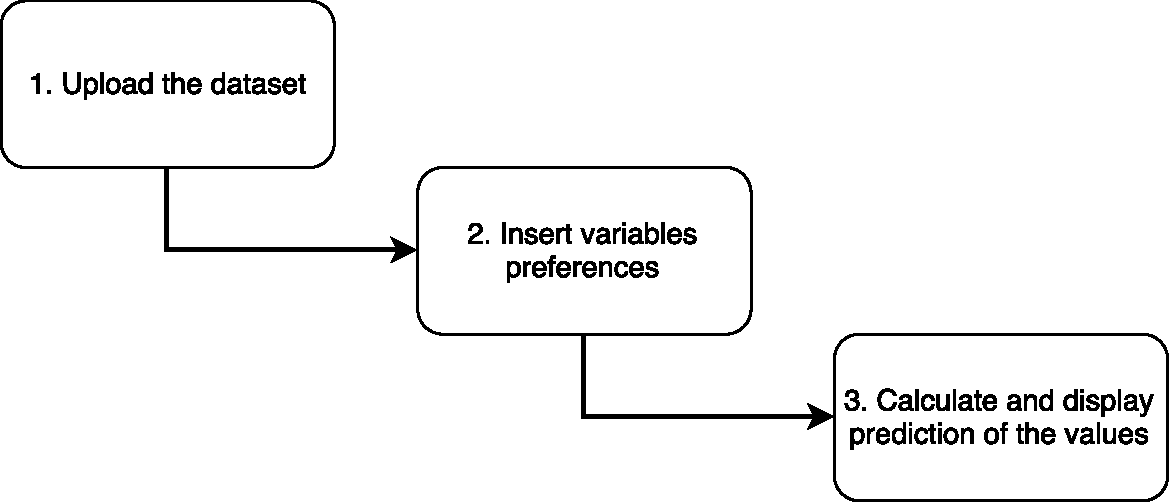
\includegraphics[width=1\textwidth]{Files/ServiceSystem.pdf}}
    \caption{Idea of the Servie System for predictions.}
\end{figure}






 % Conclusion

%
\chapter{Recommendations to future work}
\section{Dataset about single locality}
This thesis allows to have a general overview and predictions of values about the aquaculture business in Norway. 

But it would be much more useful, in particular for people into the aquaculture business, to use this system to have an overview and predictions of data provided by a single locality of aquaculture.\\
In this case the system could be used from the owner of the locality to analyze historic values and use the prediction system to have a forecast about some particular parameters.

\section{Visualization of the data}

\section{Test prediction system with a bigger dataset}

\newpage

\section{Prediction system as a service}
This system has been developed with the idea that it could become a "Service system", that is basically a configuration of technology and organizational networks designed to deliver services that satisfy the needs or wants of customers.
Since the prediction system implemented during this work is almost 100\% reusable, it could be used from people for prediction about any kind of data. 

Basically the idea is to create a web application that allows to let you upload your own dataset, choose your own preferences and prediction settings, and then the system will calculate and display prediction of the current values in the future together with the MAPE (Mean Average Percentage Error) to have an idea bout how accurate are the.\\


\begin{figure}[H]
	\centering
        \makebox[\textwidth][c]{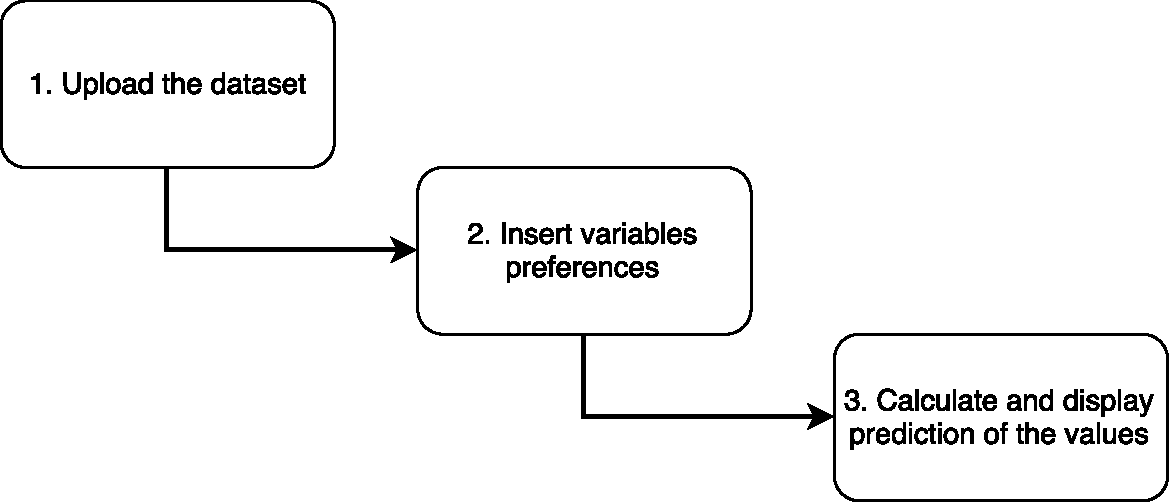
\includegraphics[width=1\textwidth]{Files/ServiceSystem.pdf}}
    \caption{Idea of the Servie System for predictions.}
\end{figure}








\chap{Bibliography}

[1] \url{http://www.fiskeridir.no/Akvakultur/Statistikk-akvakultur/Biomassestatistikk}


[2] \url{https://www.quandl.com/data/ODA/PSALM_USD-Fish-Salmon-Price}


[3] \url{http://machinelearningmastery.com/time-series-forecasting/}


[4] \url{https://github.com/Sprea22/Thesis_Latex_Doc}


[5] \url{https://github.com/Sprea22/Data_Analyzer_Python}


[6] \url{https://github.com/Sprea22/Forecasting_System_Python}

[7] \url{https://en.wikipedia.org/wiki/Data_science}

[8] \url{http://machinelearningmastery.com/time-series-forecasting/}

[9] \url{http://www.ulb.ac.be/di/map/gbonte/ftp/time_ser.pdf}

[10] \url{http://users.dma.unipi.it/~flandoli/AUTCap4.pdf}

[11] \url{http://fishpool.eu/wp-content/uploads/2016/04/final-dag.pdf}

[12] \url{mysalmon.no}

[13] \url{http://munin.uit.no/bitstream/handle/10037/5913/thesis.pdf?sequence=1}

[14] \url{http://www.indexmundi.com/commodities/?commodity=fish&months=180&currency=nok}

[15] \url{http://www.fao.org/3/a-i5555e.pdf%20} % Bibliography

%% Appendices -----------------------------------------------------



\addtocontents{toc}{\vspace{2em}} % Add a gap in the Contents, for aesthetics
\bookmarksetup{startatroot}
\lhead{\emph{Appendices}}  % Change the left side page header to "Appendices"
\appendix % Cue to tell LaTeX that the following 'chapters' are Appendices

\chap{SIA Implementation code}

\section{SIA: Imported libraries}
\label{SIA_libraries}
The library "os" is really important since provides a waay of using operating system dependent functinality.
\begin{lstlisting}
import os
\end{lstlisting}

Also the library "sys" would be very useful for test and execute the program, mainly because it allows to input directly from terminal.
\begin{lstlisting}
import sys
\end{lstlisting}

The "pylab" library will be useful for plot data.
\begin{lstlisting}
import pylab
\end{lstlisting}

The "pandas" library will be very useful for read the data from CSV dataset and setup the plot abut it.
\begin{lstlisting}
import pandas as pd
\end{lstlisting}

The "numpy" library it's used for mathematic purpose, such as calculating the correlation coefficent between two series.
\begin{lstlisting}
import numpy as np
\end{lstlisting}
 
The "pyplot" library it's used for basic graphic displaying and customization, easy to use but very efficent.
\begin{lstlisting}
import matplotlib.pyplot as pyplot
\end{lstlisting}

The library "PIL" supports many file formats, and provides powerful image processing and graphics capabilities.
\begin{lstlisting}
from PIL import Image
\end{lstlisting}

The library "fpdf" allows to generate and use PDF file.
\begin{lstlisting}
from fpdf import FPDF
\end{lstlisting}

\section{SIA section I: Total graphic for all the years}
\label{SIA_section_I}
\textbf{Code implementation:}\\
During this section of the code was used "pandas" library for read the dataset.
\begin{lstlisting}
series = pd.read_csv("Dataset.csv", usecols=[1,sys.argv[1]])
\end{lstlisting}

Then using the "pyplot" library has been possible to setup the plot of the input data.
\begin{lstlisting}
series.plot(color="blue", linewidth=1.5)
\end{lstlisting}


Thera are some settings about the axis x just to display the data in the right format, are easy to change and to costume.
\begin{lstlisting}
years = ["2005","2006","2007","2008","2009","2010",
	"2011","2012","2013","2014","2015","2016"]
x = range(144)
pyplot.xticks(np.arange(min(x), max(x)+1, 12.0), years)
pyplot.title("Total graphic from 2005 to 2016")
\end{lstlisting}

Once setted up the plot of the current data, the next step was to display the trendline of the current graphic. \\ 
The following code represent the method for calculate and display it.
\begin{lstlisting}
def trendline(x, y, col):
	z = np.polyfit(x, y, 1)
	p = np.poly1d(z)
	pylab.plot(x,p(x), c=col)
	# print "y=%.6fx+(%.6f)"%(z[0],z[1])
\end{lstlisting}	

At this point the current data values have been read again and passed to the method just impleneted above for calculating the trendline.
\begin{lstlisting}
series2 = pd.read_csv("Dataset.csv", usecols=[sys.argv[1]],
			squeeze=True)
trendline(x, seriesV.values, "red")
\end{lstlisting}

There is the possibility to save the graphic like an image and/or display it.
\begin{lstlisting}
saveFigure("_Total.jpg")
\end{lstlisting}


\section{SIA section II: Single graphics for each year}
\label{SIA_section_II}
\textbf{Code implementation:}\\
During this section of the code was used "pandas" library for read the dataset.
\begin{lstlisting}
series2 = pd.read_csv("Dataset.csv", index_col=['Month'],
			usecols=[0,1,sys.argv[1]])
\end{lstlisting}

Some initialization of variables that are going to be useful.
\begin{lstlisting}
months = ["Jan","Feb","Mar","Apr","May","Jun",
		"Jul","Aug","Sep","Oct","Nov","Dec"]
x_pos = np.arange(len(months))
test = []
j = 0
\end{lstlisting}

The following code allows the system to split the values and display them in the right way: that means that are going to be splitted for each single year and then plotted on the same graphic.
\begin{lstlisting}
for i in range(len(series2.values)):
	if j in range(12):
		test.append(series2.values[i][1])
		j = j + 1
	else:
		pyplot.plot(x_pos, test, linewidth=2, 
			alpha=0.8, 
			label = int(series2.values[i-1][0]))
		test = []
		test.append(series2.values[i][1])
		j = 1

\end{lstlisting}

These are some personalization settings that could be easily changed as you want.
\begin{lstlisting}
ax.legend(loc=4, ncol=1, fancybox=True, shadow=True)
pyplot.xticks(x_pos,months)
pyplot.xlim(0,11)
pyplot.title(sys.argv[1]+ 
		": Single year's graphic from 2005 to 2016")
\end{lstlisting}

There is the possibility to save the graphic like an image and/or display it.
\begin{lstlisting}
saveFigure("_Years.jpg")
\end{lstlisting}


\section{SIA section III: Correlation matrix between years}
\label{SIA_section_III}
\textbf{Code implementation:}\\
During this section of the code was used "pandas" library for read the dataset.
\begin{lstlisting}
series3 = pd.read_csv("Dataset.csv", index_col=['Year'],
			usecols=[0,sys.argv[1]])
\end{lstlisting}

\begin{lstlisting}
corr = []
test = []
j = 0
# Collecting the correct values to elaborate.
for i in range(len(series2.values)+1):
	if j in range(12):
		test.append(series2.values[i][1])
		j = j + 1
	else:
		corr.append(test)
		test = []
		if i in range(144):
			test.append(series2.values[i][1])
			j = 1
\end{lstlisting}

With the library "numpy" is possible to calculate the correlation coefficents between all the variables in the series just read.
\begin{lstlisting}
test = np.corrcoef(corr)
\end{lstlisting}

Setup the figure that will display the correlation matrix using the library "pypot".
\begin{lstlisting}
fig2 = pyplot.figure()
ax = fig2.add_subplot(111)
\end{lstlisting}

Creating the correlation matrix using the already calculated correlation coefficents.
\begin{lstlisting}
cax = ax.matshow(test, interpolation='nearest')
\end{lstlisting}

Settings for display the matrix in the right way, in particular for the values to display on both the axis x and y, in this case every single year from 2005 to 2016
\begin{lstlisting}
pyplot.title(sys.argv[1]+ ": Correlation between different years")
years = ["2005","2006","2007","2008","2009","2010",
	"2011","2012","2013","2014","2015","2016"]
x_pos = np.arange(len(years))
y_pos = np.arange(len(years))
pyplot.yticks(y_pos,years)
pyplot.xticks(x_pos,years)
pyplot.colorbar(cax)
\end{lstlisting}
\newpage
Adding a title to the graphic that we are going to display and also a bar that works like a legend for the colors of the matrix, allowing the reader to better understand the values reported inside the matrix.
\begin{lstlisting}
saveFigure("_Years_Matrix.jpg")
\end{lstlisting}

There is the possibility to save the correlation matrix like an image and/or display it.
\begin{lstlisting}
pyplot.savefig("OUTPUT_DIRECTORY", format="jpg")
pyplot.show()
\end{lstlisting}


\section{SIA section IV: Correlation matrix between months}
\label{SIA_section_IV}
\textbf{Code implementation:}\\
During this section of the code was used "pandas" library for read the dataset.
\begin{lstlisting}
series4 = pd.read_csv("Dataset.csv", usecols=[0,1,sys.argv[1]])
\end{lstlisting}

\begin{lstlisting}
corr = []
for Month, Year in series4.groupby(["Month"], sort=False):
	corr.append(Year[sys.argv[1]].values)
\end{lstlisting}
	
With the library "numpy" is possible to calculate the correlation coefficents between all the variables in the series just read.
\begin{lstlisting}
test = np.corrcoef(series4.values)
\end{lstlisting}

Setup the figure that will display the correlation matrix using the library "pypot".
\begin{lstlisting}
fig2 = pyplot.figure()
ax = fig2.add_subplot(111)
\end{lstlisting}

Creating the correlation matrix using the already calculated correlation coefficents.
\begin{lstlisting}
cax = ax.matshow(test, interpolation='nearest')
\end{lstlisting}

Settings for display the matrix in the right way, in particular for the values to display on both the axis x and y, in this case every single months of the year.
\begin{lstlisting}
months = ["Jan","Feb","Mar","Apr","May","Jun",
	"Jul","Aug","Sep","Oct","Nov","Dec"]
x_pos = np.arange(len(months))
y_pos = np.arange(len(months))
pyplot.yticks(y_pos,months)
pyplot.xticks(x_pos,months)
\end{lstlisting}
Adding a title to the graphic that we are going to display and also a bar that works like a legend for the colors of the matrix, allowing the reader to better understand the values reported inside the matrix.
\begin{lstlisting}
pyplot.title("Correlation between different months")
pyplot.colorbar(cax)
\end{lstlisting}

There is the possibility to save the correlation matrix like an image and/or display it.
\begin{lstlisting}
saveFigure("_Months_Matrix.jpg")
pyplot.show()
\end{lstlisting}

\section{SIA section V: Single overview}
\label{SIA_section_V}
\textbf{Code implementation:}\\
create\_single\_overview() : this method will use the "Image" library for autogenerate a collage of the current input's graphics and save it like an overview image. The content of the params will basically decide how the "Current input overview image" will looks like.

It uses each single "current input overview image" of all the inputs and the "correlation matrix between all the inputs image" for combine them in a unique "total overview" and save it using the PDF format.

\begin{lstlisting}
listofimages=["CURRENT_INPUT_TOTAL_GRAPHIC",
            "CURRENT_INPUT_YEARS_MATRIX", 
            "CURRENT_INPUT_YEARS_GRAPHIC",
            "CURRENT_INPUT_MONTHS_MATRIX"]
            
create_single_overview(params1, listofimages)
create_single_overview(params2, listofimages)
\end{lstlisting}


The "create\_single\_overview" method has basically this structured, and then its configuration depends from the input data and from the preferences.
\begin{lstlisting}
def create_single_overview(cols, rows ,
			width, height, listofimages):
    thumbnail_width = width//cols
    thumbnail_height = height//rows
    size = thumbnail_width, thumbnail_height
    new_im = Image.new('RGB', (width, height))
    ims = []
    for p in listofimages:
        im = Image.open(p)
        im.thumbnail(size)
        ims.append(im)
    i = 0
    x = 0
    y = 0
    for col in range(cols):
        for row in range(rows):
            new_im.paste(ims[i], (x, y))
            i += 1
            y += thumbnail_height
        x += thumbnail_width
        y = 0
    new_im.save(SINGLE_OVERVIEW_IMAGE")
	new_im.show()
\end{lstlisting}
 % SIA Implementation code

\chap{MIA Implementation code}
\label{MIA_Implementation}
\section{MIA: Imported libraries}
\label{MIA_Libraries}
The "pandas" library will be very useful for read the data from CSV dataset and setup the plot abut it.
\begin{lstlisting}
import pandas as pd
\end{lstlisting}

The "numpy" library it's used for mathematic purpose, such as calculating the correlation coefficent between two series.
\begin{lstlisting}
import numpy as np
\end{lstlisting}

 
The "pyplot" library it's used for basic graphic displaying and customization, easy to use but very efficent.
\begin{lstlisting}
import matplotlib.pyplot as pyplot
\end{lstlisting}

\section{MIA: Implementation}
\textbf{Code implementation:}\\
First of all, we are going to use the "pandas" library for read the dataset.
\begin{lstlisting}
series3 = pd.read_csv("TOTAL_DATASET_DIRECTORY", 
	index_col=['Input'], header=0)
\end{lstlisting}

Then with the library "numpy" is possible to calculate the correlation coefficents between all the variables just read above.
\begin{lstlisting}
test = np.corrcoef(series3.values)
\end{lstlisting}

Setup the figure that will display the correlation matrix using the library "pyplot".
\begin{lstlisting}
fig2 = pyplot.figure()
ax = fig2.add_subplot(111)
\end{lstlisting}

Creating the correlationg matrix using the already calculated correlation coefficents.
\begin{lstlisting}
cax = ax.matshow(test, interpolation='nearest')
\end{lstlisting}

Settings for display the matrix in the right way, in particular for the values to display on both the axis x and y, in this case every single input.
\begin{lstlisting}
inputs = ["Cages", "Feed", "Number", "Restock",
	"Local", "Withdr", "Biomass", "Price"]
x_pos = np.arange(len(inputs))
y_pos = np.arange(len(inputs))
pyplot.yticks(y_pos,inputs)
pyplot.xticks(x_pos,inputs)
\end{lstlisting}

Adding a title to the graphic that we are going to display and also a ba that works like a legend for the colors of the matrix, allowing the reader to better understand the values reported inside the matrix.
\begin{lstlisting}
pyplot.title("Correlation between different inputs 
		about data from 2005 to 2016")
pyplot.colorbar(cax)
\end{lstlisting}

In the end, using again the library "pyplot", there is the possibility to save the correlation matrix graphic like an image and/or display it.
\begin{lstlisting}
pyplot.savefig("OUTPUT_DIRECTORY")
\end{lstlisting}

\begin{lstlisting}
series = pd.read_csv("TRENDLINES_VALUES_DOCUMENT",
	 header=0, usecols=["Norm Ang Coeffs"])
series.plot(kind="barh")
pyplot.savefig("OUTPUT_DIRECTORY")

create_total_overview()
\end{lstlisting}

\begin{lstlisting}
pyplot.show()
\end{lstlisting}

 % MIA Implementation code

\chap{Prediction System Implementation code}
\section{Evaluating System}
\section{Training System}
\section{Future Prediction System}

 % Prediction System Implementation code

\end{document}  % The End
%% ----------------------------------------------------------------